% บทที่ 3 คู่มือการติดตั้งระบบ
บทนี้อธิบายลำดับการเตรียมเครื่องมือ ติดตั้ง และตั้งค่าระบบ Pacegasus
สำหรับผู้ติดตั้งหรือผู้พัฒนาที่ต้องการนำระบบไปใช้งาน

\section{การเตรียมความพร้อมก่อนติดตั้ง}
ตรวจสอบอุปกรณ์ เครื่องมือ และบัญชีบริการที่จำเป็นก่อนเริ่มติดตั้งระบบ
% TODO: เพิ่มรายการไฟล์ต้นฉบับ เครื่องมือ และบัญชีที่ต้องใช้จริง

\section{การติดตั้งเครื่องมือที่จำเป็น}
\subsection{การติดตั้ง Flutter SDK}
% TODO: เพิ่มขั้นตอนติดตั้ง การตั้งค่า PATH และภาพตรวจสอบความพร้อม

\subsection{การติดตั้ง Visual Studio Code}
Visual Studio Code เป็นโปรแกรมสำหรับเปิดและแก้ไขไฟล์โค้ดของโครงการ
ขั้นตอนต่อไปนี้เป็นการติดตั้งบนระบบปฏิบัติการ Windows
\begin{enumerate}[label=\arabic*)]
    \item ดาวน์โหลดไฟล์ติดตั้ง Visual Studio Code จากเว็บไซต์
    \url{https://code.visualstudio.com/} โดยเลือกตัวติดตั้งสำหรับ Windows
    \item เปิดไฟล์ติดตั้งที่ดาวน์โหลดมา อ่านข้อตกลงการใช้งาน
    แล้วเลือก I accept the agreement เพื่อยอมรับเงื่อนไข
    จากนั้นกดปุ่ม Next เพื่อดำเนินการต่อ
\end{enumerate}
% ภาพที่ผู้ใช้ส่ง: image(20261026-053108).png
\IfFileExists{images/installation/vscode-license.png}{%
\begin{figure}[H]
    \centering
    \includegraphics[width=0.85\textwidth,height=0.42\textheight,keepaspectratio]{images/installation/vscode-license.png}
    \caption{การอ่านและยอมรับข้อตกลงการติดตั้ง Visual Studio Code}
    \label{fig:vscode-license}
\end{figure}
}{}
\begin{enumerate}[label=\arabic*),start=3]
    \item ดำเนินการตามหน้าต่างติดตั้งจนถึงหน้าตรวจสอบรายละเอียดก่อนติดตั้ง
    ตรวจสอบรายละเอียด แล้วกดปุ่ม Install เพื่อเริ่มติดตั้งโปรแกรม
\end{enumerate}
% ภาพที่ผู้ใช้ส่ง: image(20261026-053117).png
\IfFileExists{images/installation/vscode-install.png}{%
\begin{figure}[H]
    \centering
    \includegraphics[width=0.85\textwidth,height=0.42\textheight,keepaspectratio]{images/installation/vscode-install.png}
    \caption{การตรวจสอบรายละเอียดและเริ่มติดตั้ง Visual Studio Code}
    \label{fig:vscode-install}
\end{figure}
}{}


\subsection{การติดตั้ง Node.js}
ขั้นตอนต่อไปนี้เป็นการติดตั้ง Node.js บนระบบปฏิบัติการ Windows
และตรวจสอบค่า Path เพื่อให้เรียกใช้งานจากหน้าต่างคำสั่งได้
\begin{enumerate}[label=\arabic*)]
    \item ดาวน์โหลดไฟล์ติดตั้งจาก \url{https://nodejs.org/en/download}
    โดยเลือกตัวติดตั้งสำหรับ Windows ให้ตรงกับสถาปัตยกรรมของเครื่อง
    \item เปิดไฟล์ติดตั้งที่ดาวน์โหลดมา อ่านข้อตกลงการใช้งาน
    แล้วเลือก I accept the terms in the License Agreement
    จากนั้นกด Next เพื่อดำเนินการต่อ
    \item ดำเนินการตามหน้าต่างติดตั้งจนถึงหน้า Ready to install Node.js
    ตรวจสอบรายละเอียด แล้วกด Install เพื่อเริ่มติดตั้ง
    รอจนติดตั้งเสร็จและปิดหน้าต่างติดตั้ง
\end{enumerate}
% ภาพต้นฉบับ: image(20261026-053259).png
\IfFileExists{images/installation/node-license.png}{%
\begin{figure}[H]
    \centering
    \includegraphics[width=0.85\textwidth,height=0.42\textheight,keepaspectratio]{images/installation/node-license.png}
    \caption{การยอมรับข้อตกลงการติดตั้ง Node.js}
    \label{fig:node-license}
\end{figure}
}{}

% ภาพต้นฉบับ: image(20261026-053307).png
\IfFileExists{images/installation/node-install.png}{%
\begin{figure}[H]
    \centering
    \includegraphics[width=0.85\textwidth,height=0.42\textheight,keepaspectratio]{images/installation/node-install.png}
    \caption{การตรวจสอบรายละเอียดและเริ่มติดตั้ง Node.js}
    \label{fig:node-install}
\end{figure}
}{}

\subsubsection{การตั้งค่า Path ของ Node.js}
\begin{enumerate}[label=\arabic*)]
    \item เปิดหน้าต่าง System Properties เลือกแท็บ Advanced
    แล้วกดปุ่ม Environment Variables
    \item ในส่วน System variables เลือกตัวแปร Path แล้วกด Edit
    \item ตรวจสอบว่ามีตำแหน่งติดตั้ง Node.js อยู่ในรายการแล้วหรือไม่
    หากมีอยู่แล้ว ไม่ต้องเพิ่มรายการซ้ำ
    หากยังไม่มี ให้กด New และกรอกตำแหน่งโฟลเดอร์ที่ติดตั้ง Node.js
    เช่น \verb|C:\Program Files\nodejs\|
    โดยใช้ตำแหน่งจริงที่เลือกไว้ระหว่างติดตั้ง
    \item กด OK เพื่อบันทึกค่าในหน้าต่างแก้ไข Path
    จากนั้นกด OK ในหน้าต่าง Environment Variables และ System Properties
\end{enumerate}
% ภาพต้นฉบับ: image(20261026-053442).png
\IfFileExists{images/installation/node-system-properties.png}{%
\begin{figure}[H]
    \centering
    \includegraphics[width=0.85\textwidth,height=0.42\textheight,keepaspectratio]{images/installation/node-system-properties.png}
    \caption{แท็บ Advanced ในหน้าต่าง System Properties}
    \label{fig:node-system-properties}
\end{figure}
}{}

% ภาพต้นฉบับ: image(20261026-053803).png
\IfFileExists{images/installation/node-environment.png}{%
\begin{figure}[H]
    \centering
    \includegraphics[width=0.85\textwidth,height=0.42\textheight,keepaspectratio]{images/installation/node-environment.png}
    \caption{หน้าต่าง Environment Variables และส่วน System variables}
    \label{fig:node-environment}
\end{figure}
}{}

% ภาพต้นฉบับ: image(20261026-053726).png
\IfFileExists{images/installation/node-path.png}{%
\begin{figure}[H]
    \centering
    \includegraphics[width=0.85\textwidth,height=0.42\textheight,keepaspectratio]{images/installation/node-path.png}
    \caption{การตรวจสอบรายการ Path ของ Node.js}
    \label{fig:node-path}
\end{figure}
}{}

% ภาพต้นฉบับ: image(20261026-053735).png
\IfFileExists{images/installation/node-path-save.png}{%
\begin{figure}[H]
    \centering
    \includegraphics[width=0.85\textwidth,height=0.42\textheight,keepaspectratio]{images/installation/node-path-save.png}
    \caption{การเพิ่มตำแหน่ง Node.js และบันทึกค่า Path}
    \label{fig:node-path-save}
\end{figure}
}{}

\subsubsection{การตรวจสอบหลังติดตั้ง}
เปิด Command Prompt หรือ Terminal ใหม่ แล้วตรวจสอบด้วยคำสั่งต่อไปนี้
\begin{verbatim}
node --version
npm --version
\end{verbatim}
หากแสดงหมายเลขรุ่นของทั้งสองคำสั่ง แสดงว่าสามารถเรียกใช้งาน Node.js และ npm ได้

\subsection{การเตรียมอุปกรณ์สำหรับทดสอบ}
% TODO: เพิ่มขั้นตอนเตรียมอุปกรณ์จริงหรือโปรแกรมจำลอง พร้อมภาพประกอบ

\section{การติดตั้งไฟล์โครงการ}
% TODO: เพิ่มขั้นตอนรับไฟล์โครงการ เปิดโฟลเดอร์ และติดตั้งส่วนประกอบที่จำเป็น

\section{การตั้งค่า Supabase}
ภาพประกอบส่วนนี้แสดงการเลือกโครงการที่มีอยู่แล้ว
และการคัดลอกค่าการเชื่อมต่อสำหรับนำไปตั้งค่าในระบบ Pacegasus

\subsection{การเลือกองค์กรและโครงการ}
\begin{samepage}
\noindent\textbf{ขั้นตอนที่ 1} เข้าสู่บัญชี Supabase แล้วเลือกองค์กรที่ใช้สำหรับระบบ Pacegasus ตามกรอบสีแดง
\begin{figure}[H]
    \centering
    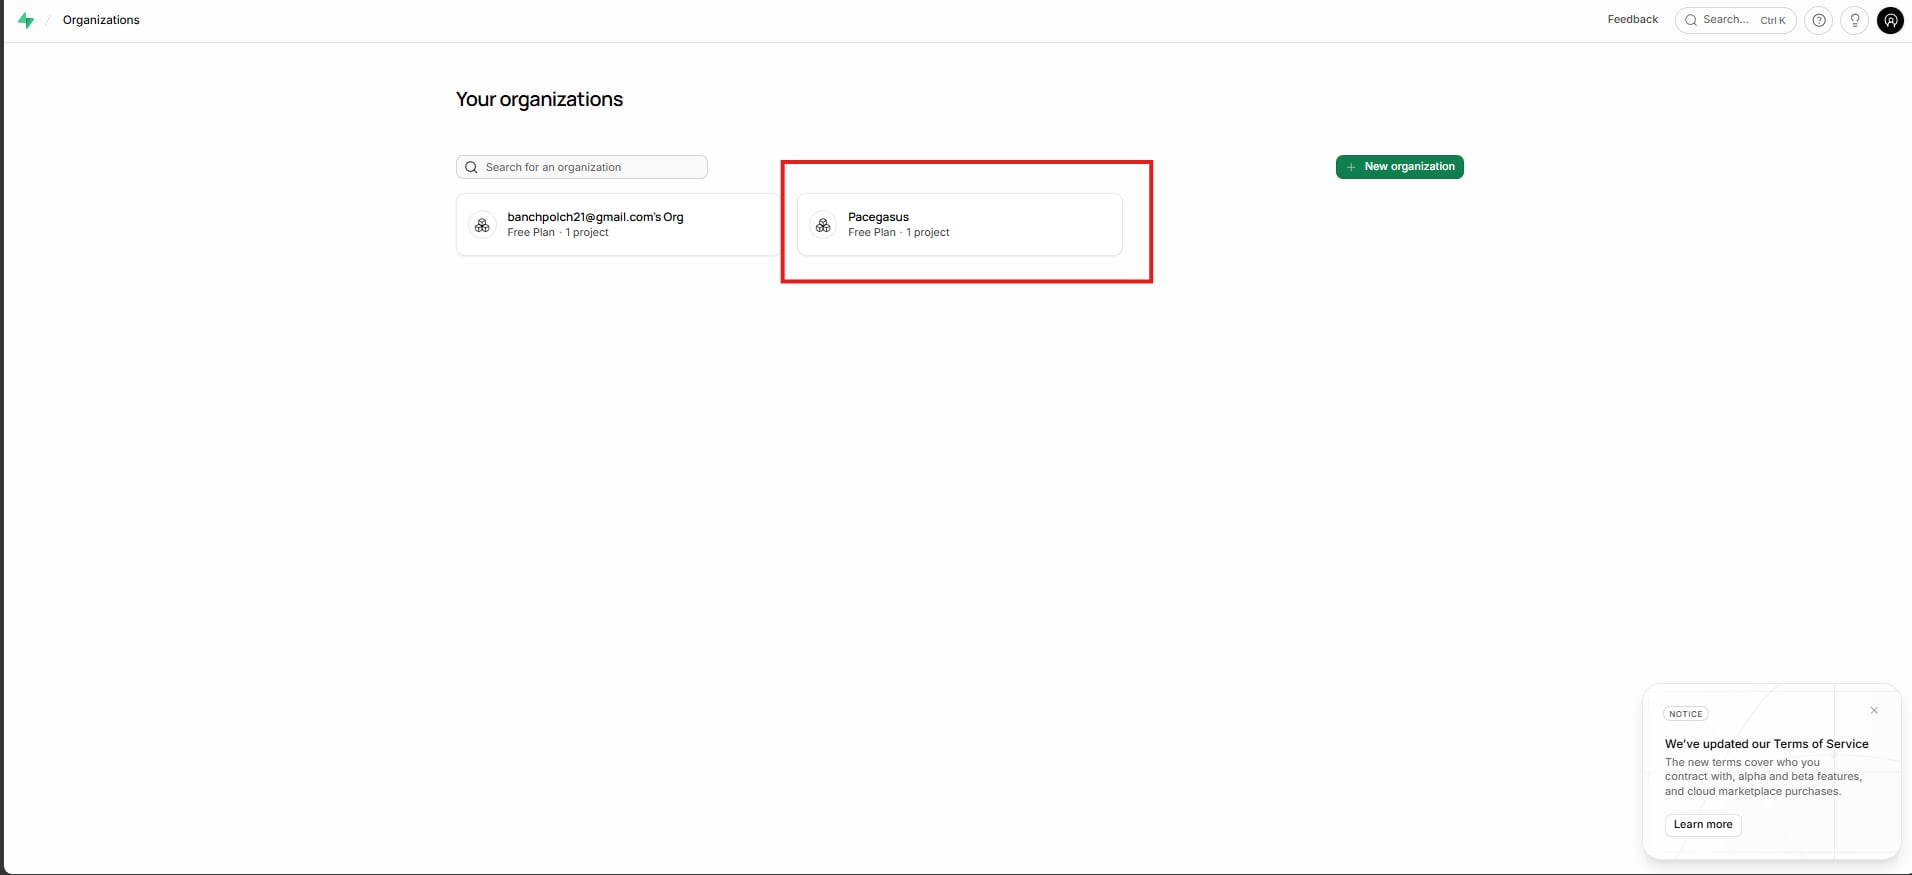
\includegraphics[width=\textwidth,height=0.30\textheight,keepaspectratio]{images/auth/auth-10.jpg}
    \caption{การเลือกองค์กรใน Supabase}
    \label{fig:auth-supabase-organization}
\end{figure}
\end{samepage}

\begin{samepage}
\noindent\textbf{ขั้นตอนที่ 2} ในหน้า Projects เลือกโครงการที่ต้องการเชื่อมต่อกับแอปพลิเคชัน
\begin{figure}[H]
    \centering
    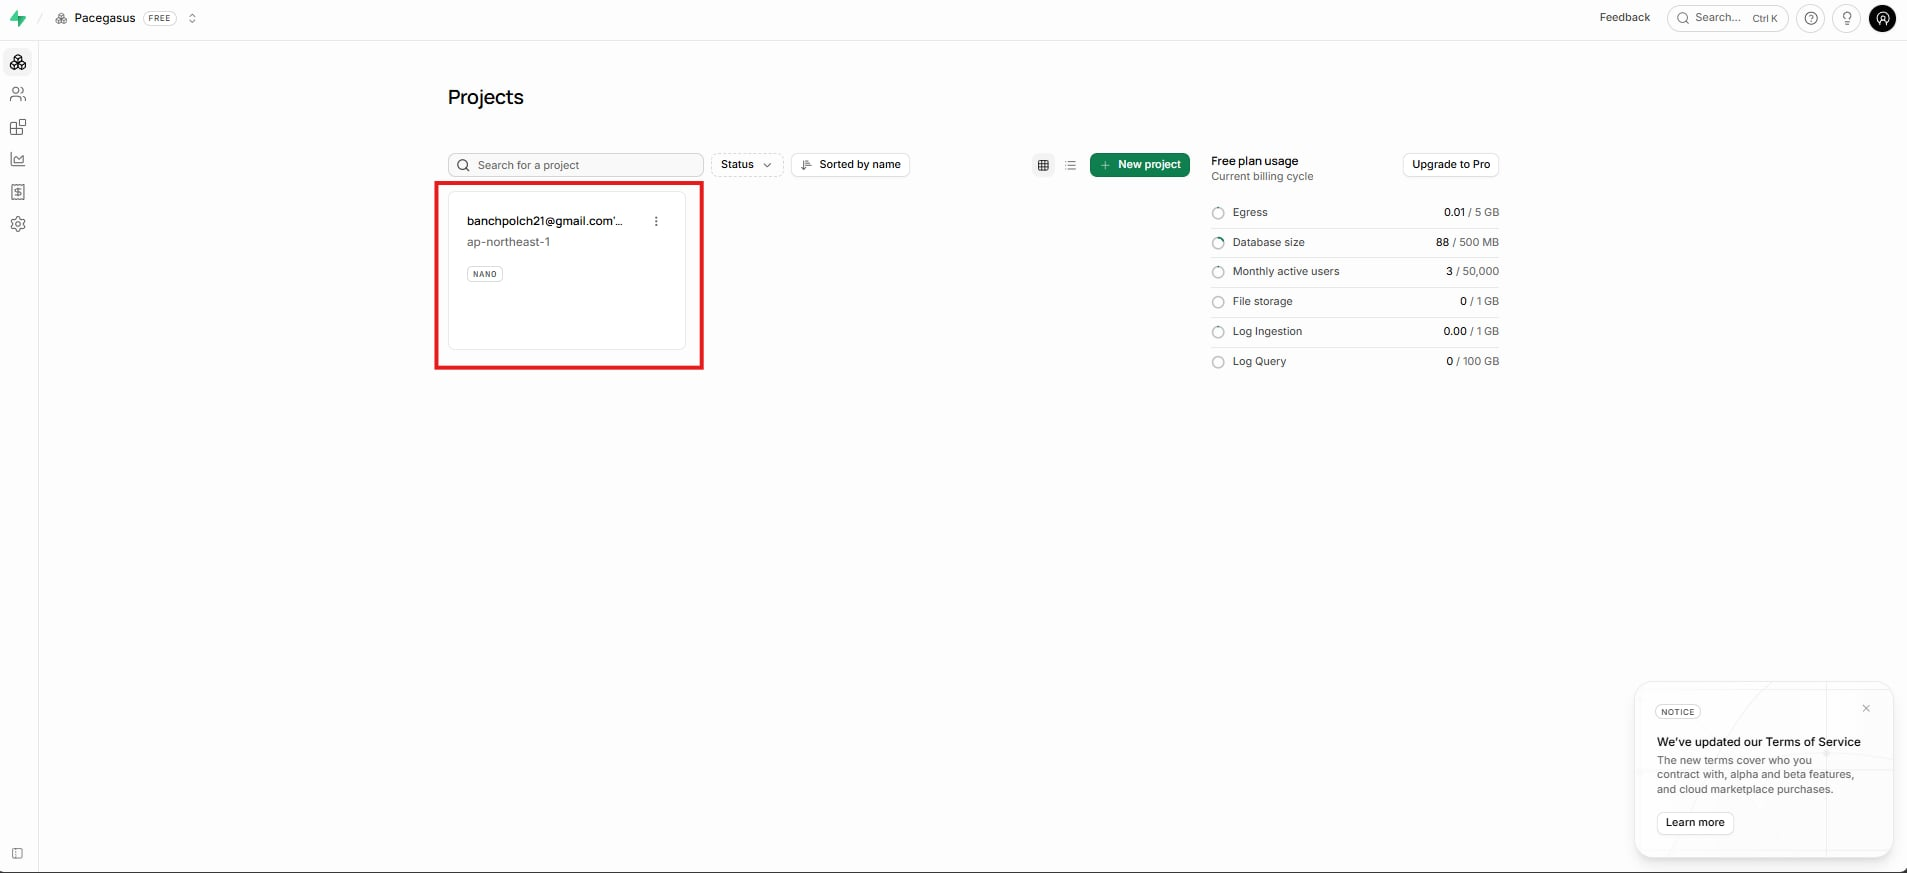
\includegraphics[width=\textwidth,height=0.30\textheight,keepaspectratio]{images/auth/auth-08.jpg}
    \caption{การเลือกโครงการใน Supabase}
    \label{fig:auth-supabase-project}
\end{figure}
\end{samepage}

\subsection{การคัดลอก Project URL และ Publishable Key}
\begin{samepage}
\noindent\textbf{ขั้นตอนที่ 3} เมื่อเข้าสู่หน้าโครงการ ให้กดปุ่ม Copy ข้างที่อยู่ของโครงการเพื่อแสดงรายการค่าที่คัดลอกได้
\begin{figure}[H]
    \centering
    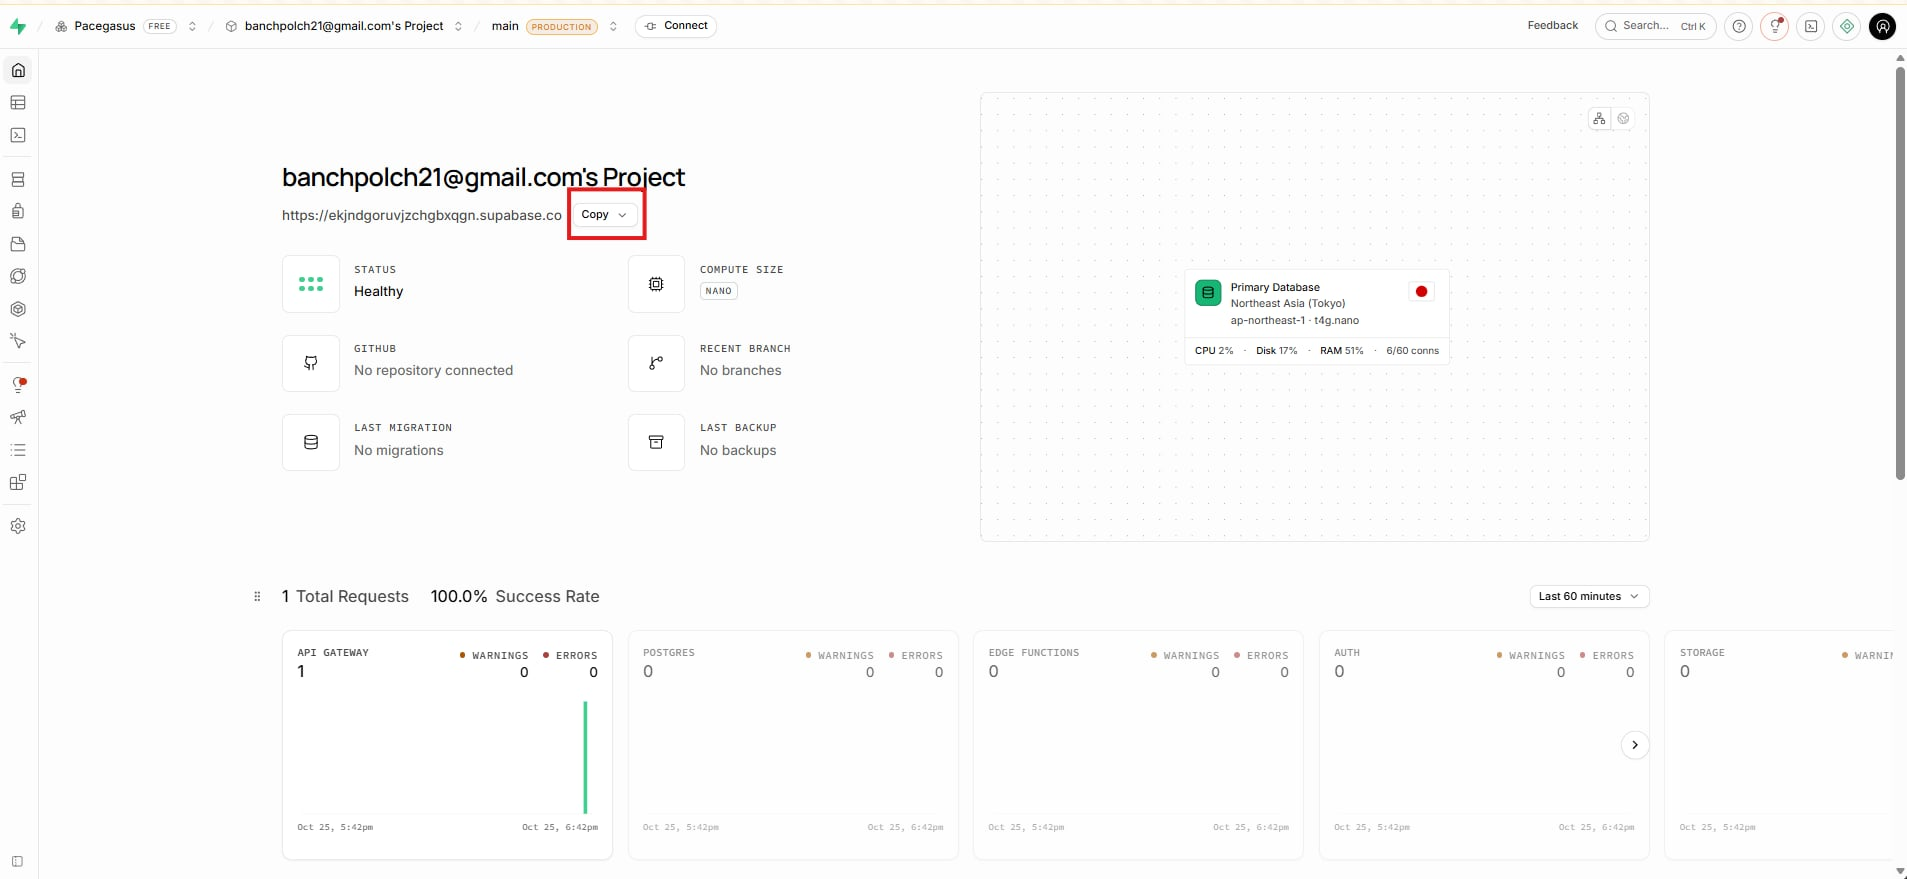
\includegraphics[width=\textwidth,height=0.30\textheight,keepaspectratio]{images/auth/auth-12.jpg}
    \caption{การเปิดเมนูคัดลอกค่าการเชื่อมต่อ Supabase}
    \label{fig:auth-supabase-copy}
\end{figure}
\end{samepage}

\begin{samepage}
\noindent\textbf{ขั้นตอนที่ 4} เลือกรายการ Project URL เพื่อคัดลอกที่อยู่ของโครงการ สำหรับนำไปกำหนดในค่าการเชื่อมต่อของระบบ
\begin{figure}[H]
    \centering
    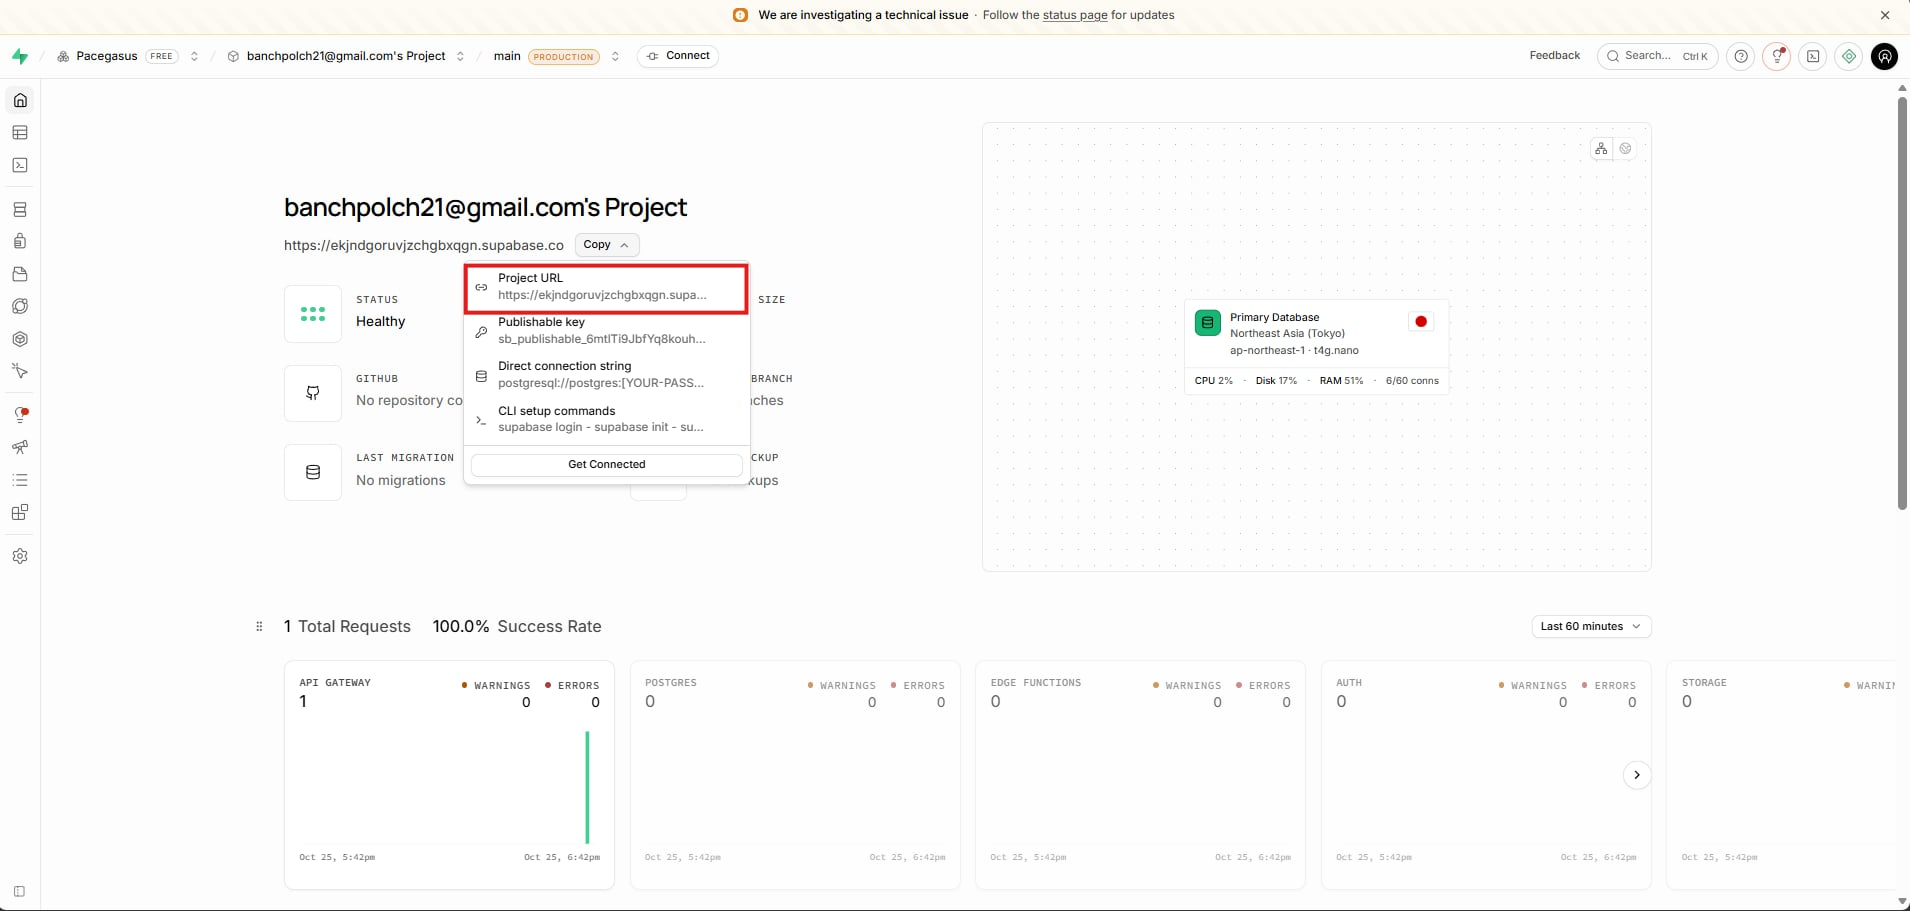
\includegraphics[width=\textwidth,height=0.30\textheight,keepaspectratio]{images/auth/auth-04.jpg}
    \caption{การคัดลอก Project URL}
    \label{fig:auth-supabase-url}
\end{figure}
\end{samepage}

\begin{samepage}
\noindent\textbf{ขั้นตอนที่ 5} เปิดเมนู Copy อีกครั้ง แล้วเลือกรายการ Publishable key เพื่อคัดลอกคีย์สำหรับการเชื่อมต่อฝั่งแอปพลิเคชัน
\begin{figure}[H]
    \centering
    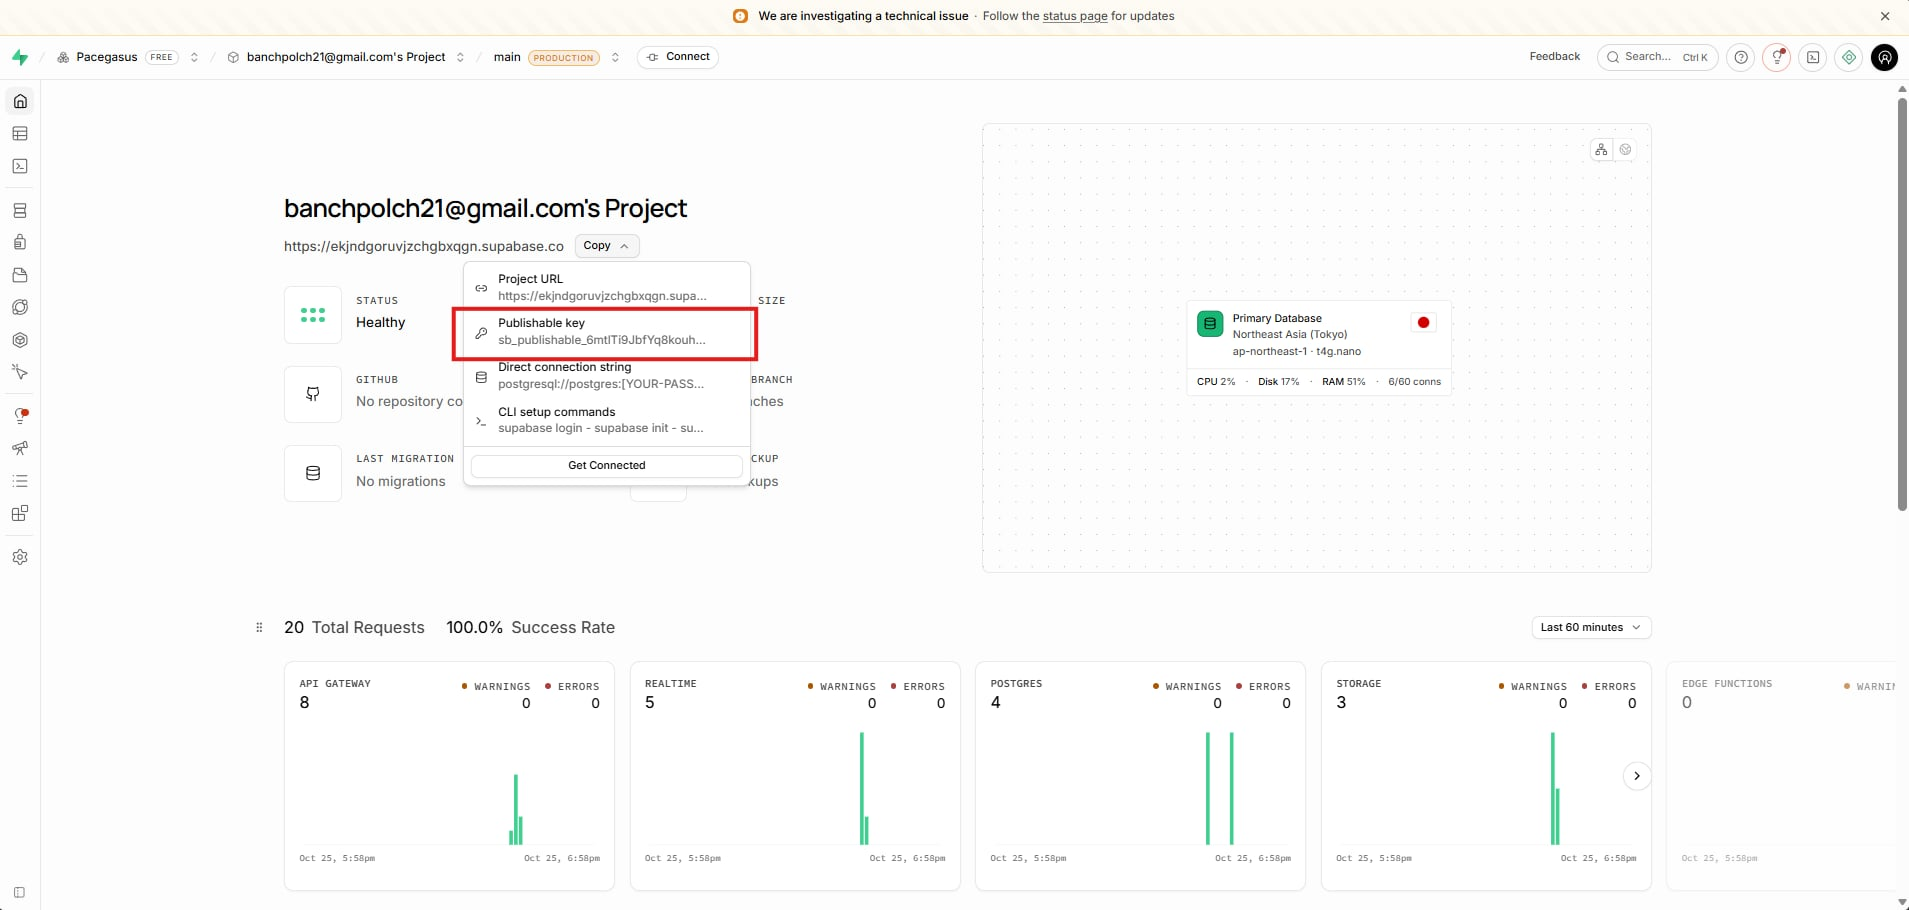
\includegraphics[width=\textwidth,height=0.30\textheight,keepaspectratio]{images/auth/auth-14.jpg}
    \caption{การคัดลอก Publishable Key}
    \label{fig:auth-supabase-publishable}
\end{figure}
\end{samepage}

\subsection{การนำค่าเชื่อมต่อไปกำหนดในระบบ}
นำ Project URL และ Publishable Key ที่คัดลอกได้ไปกำหนดในส่วนตั้งค่าการเชื่อมต่อ Supabase ของโครงการ
โดยใช้ค่าของโครงการที่ผู้ติดตั้งเลือกไว้
% TODO: เพิ่มภาพไฟล์ตั้งค่าและชื่อตัวแปรจริงสำหรับ Project URL และ Publishable Key
% TODO: เพิ่มขั้นตอนเตรียมโครงสร้างฐานข้อมูลของระบบเมื่อมีไฟล์และภาพประกอบ

\section{การตั้งค่า Google Authentication}
ภาพประกอบส่วนนี้แสดงการเข้า Google Cloud Console
เลือกโครงการ และเตรียม OAuth Client สำหรับ Web application และ Android

\subsection{การเข้าสู่ Google Cloud Console และเลือกโครงการ}
\begin{samepage}
\noindent\textbf{ขั้นตอนที่ 1} เปิดหน้า Google Cloud Console แล้วกด Go to my console จากนั้นเข้าสู่ระบบด้วยบัญชีที่ใช้ดูแลโครงการ
\begin{figure}[H]
    \centering
    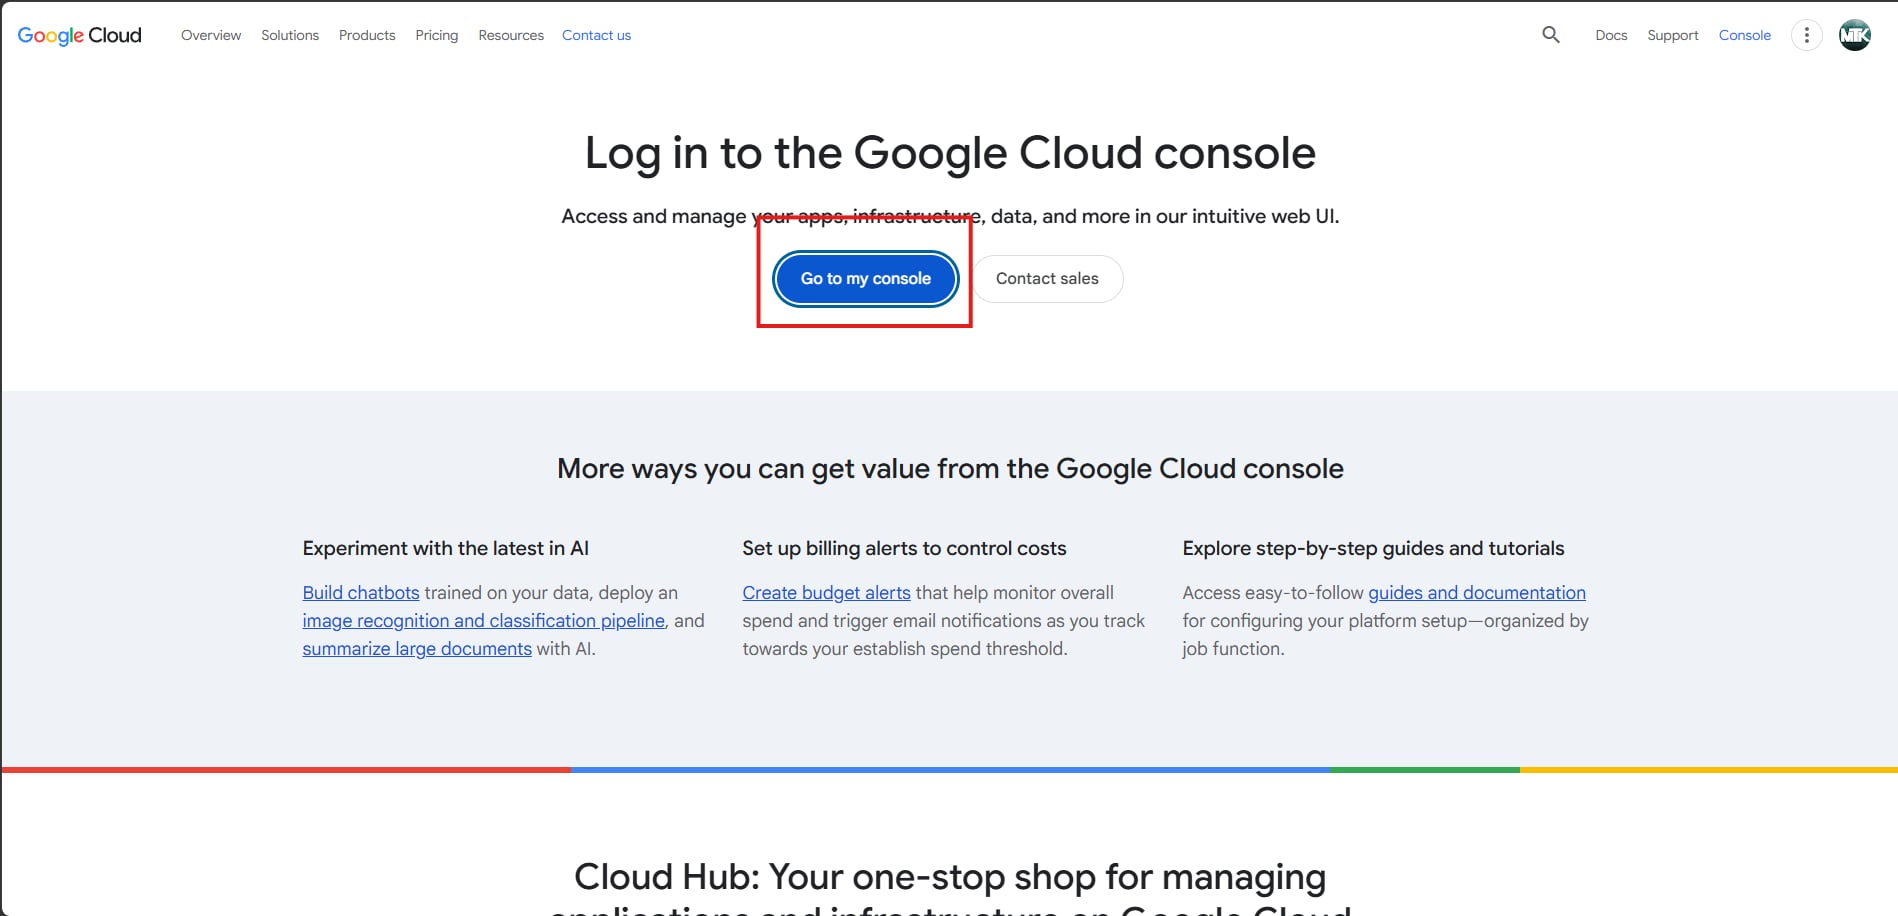
\includegraphics[width=\textwidth,height=0.30\textheight,keepaspectratio]{images/auth/auth-11.jpg}
    \caption{การเข้าสู่ Google Cloud Console}
    \label{fig:auth-google-console}
\end{figure}
\end{samepage}

\begin{samepage}
\noindent\textbf{ขั้นตอนที่ 2} กดชื่อโครงการบริเวณด้านบนของหน้า เพื่อเปิดรายการโครงการที่บัญชีสามารถเข้าถึงได้
\begin{figure}[H]
    \centering
    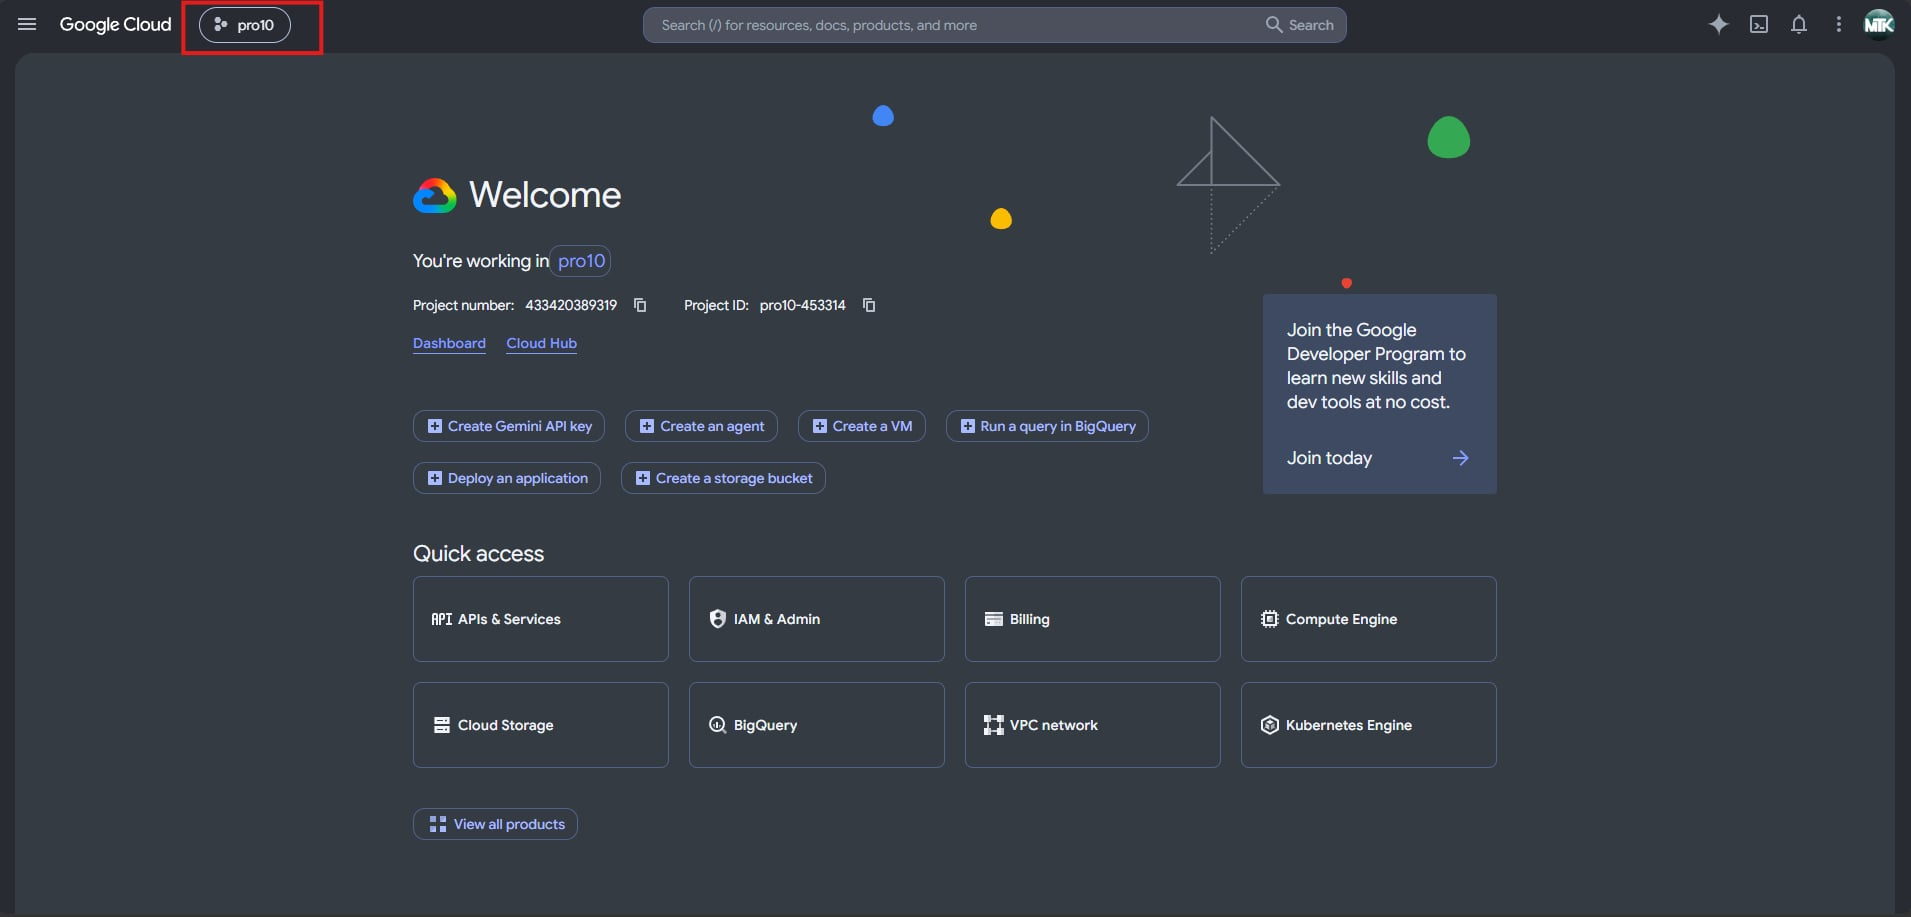
\includegraphics[width=\textwidth,height=0.30\textheight,keepaspectratio]{images/auth/auth-03.jpg}
    \caption{การเปิดรายการโครงการ Google Cloud}
    \label{fig:auth-google-project-menu}
\end{figure}
\end{samepage}

\begin{samepage}
\noindent\textbf{ขั้นตอนที่ 3} เลือกโครงการที่ใช้สำหรับตั้งค่าการเข้าสู่ระบบของ Pacegasus โดยโครงการในภาพเป็นตัวอย่างของผู้จัดทำ
\begin{figure}[H]
    \centering
    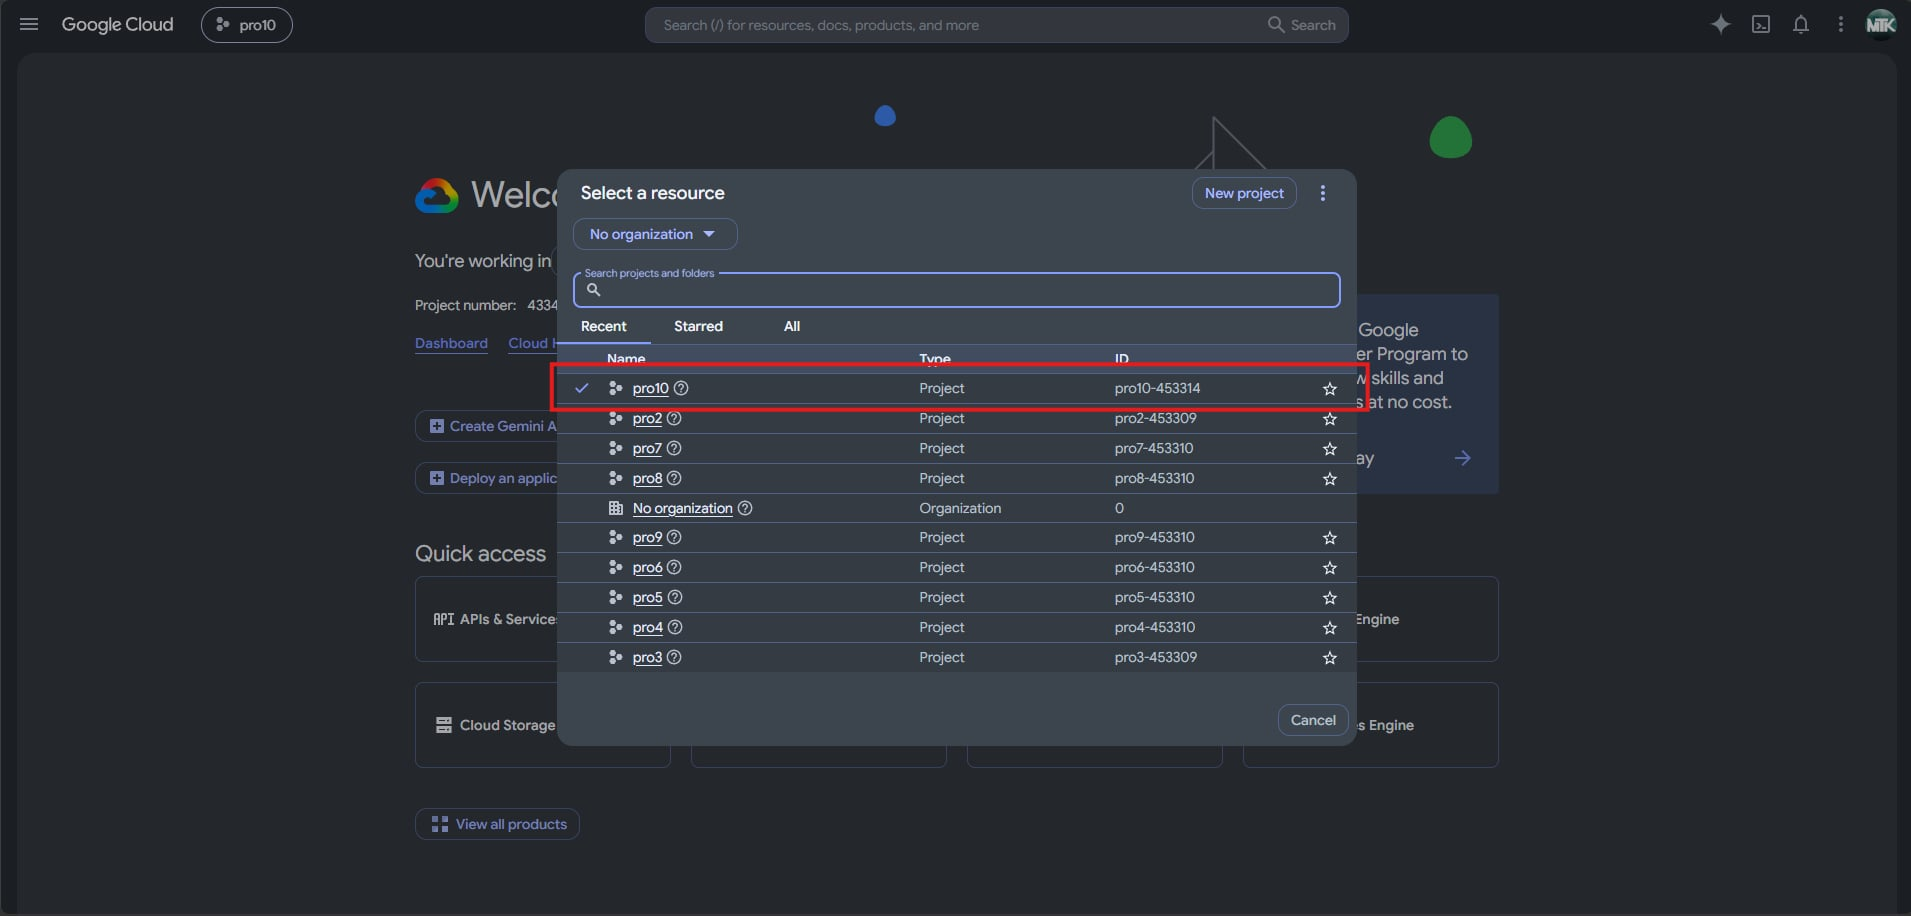
\includegraphics[width=\textwidth,height=0.30\textheight,keepaspectratio]{images/auth/auth-07.jpg}
    \caption{การเลือกโครงการ Google Cloud}
    \label{fig:auth-google-select-project}
\end{figure}
\end{samepage}

\begin{samepage}
\noindent\textbf{ขั้นตอนที่ 4} ที่หน้าโครงการ เลือกเมนู APIs \& Services ตามกรอบสีแดง
\begin{figure}[H]
    \centering
    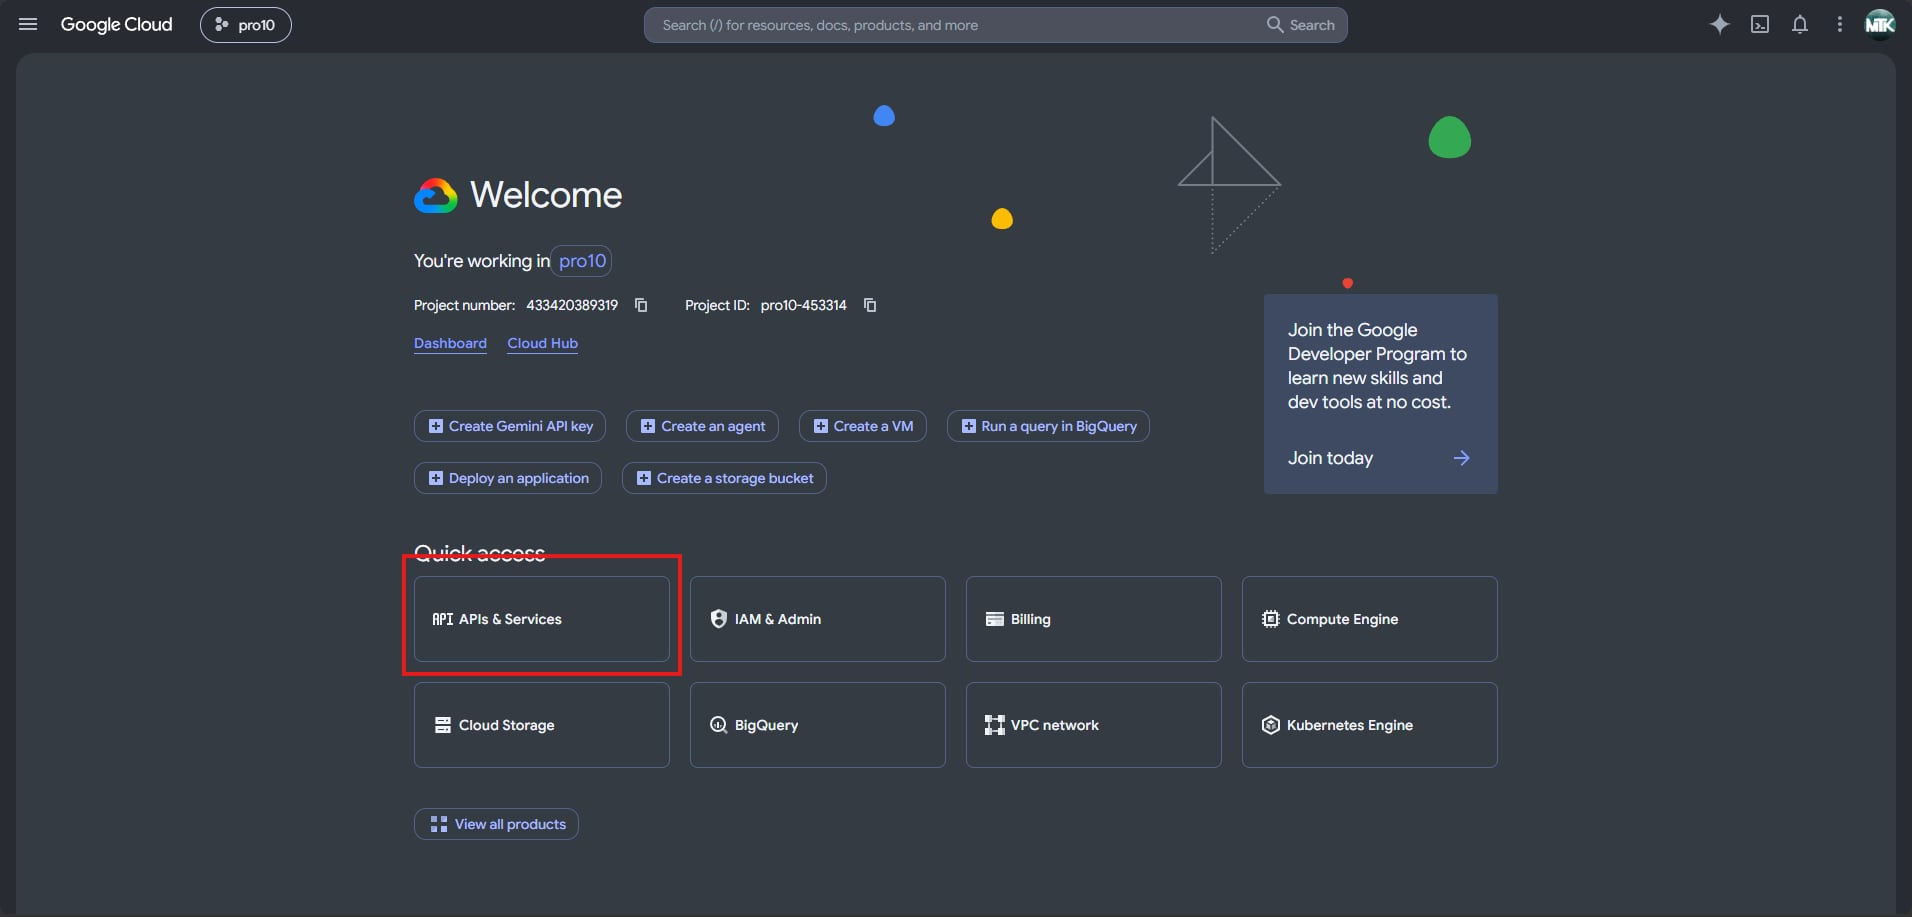
\includegraphics[width=\textwidth,height=0.30\textheight,keepaspectratio]{images/auth/auth-13.jpg}
    \caption{การเปิดหน้า APIs และ Services}
    \label{fig:auth-google-api-services}
\end{figure}
\end{samepage}

\begin{samepage}
\noindent\textbf{ขั้นตอนที่ 5} เลือกเมนู OAuth consent screen เพื่อเข้าสู่ส่วนตั้งค่าการยืนยันตัวตนของแอปพลิเคชัน
\begin{figure}[H]
    \centering
    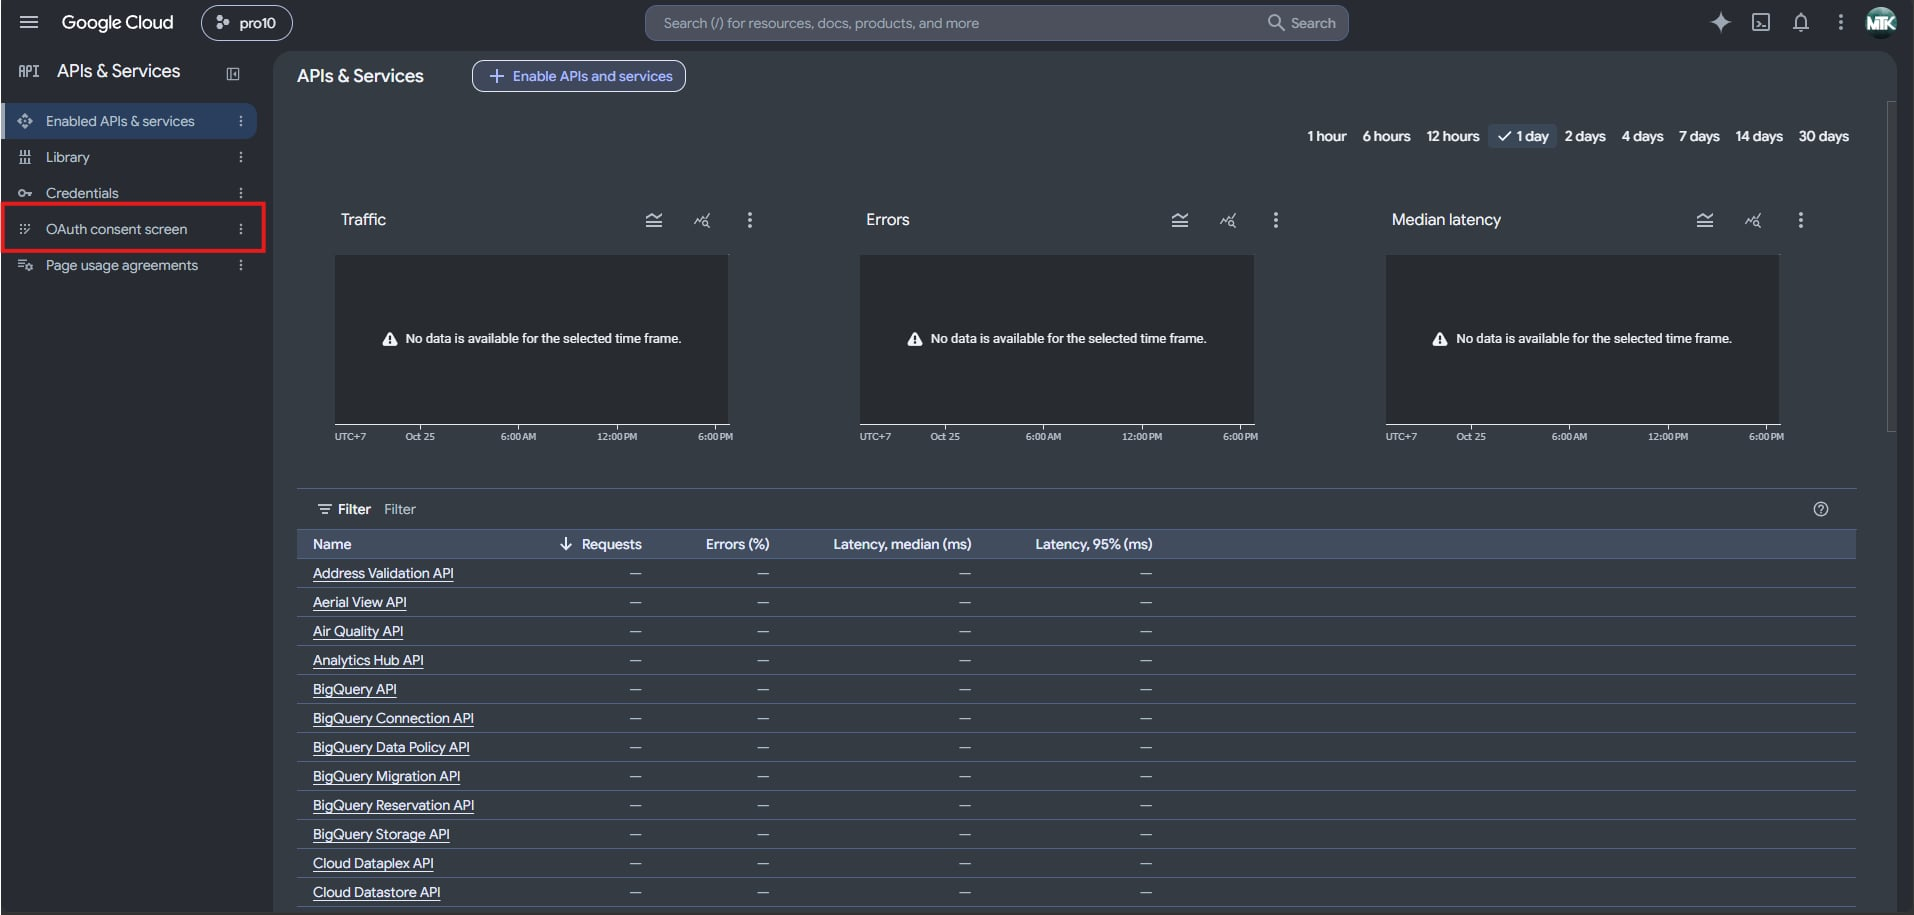
\includegraphics[width=\textwidth,height=0.30\textheight,keepaspectratio]{images/auth/auth-09.jpg}
    \caption{การเข้าสู่ส่วน OAuth consent screen}
    \label{fig:auth-google-consent}
\end{figure}
\end{samepage}

\begin{samepage}
\noindent\textbf{ขั้นตอนที่ 6} ในหน้า Google Auth Platform เลือกเมนู Clients เพื่อจัดการ OAuth Client ของโครงการ
\begin{figure}[H]
    \centering
    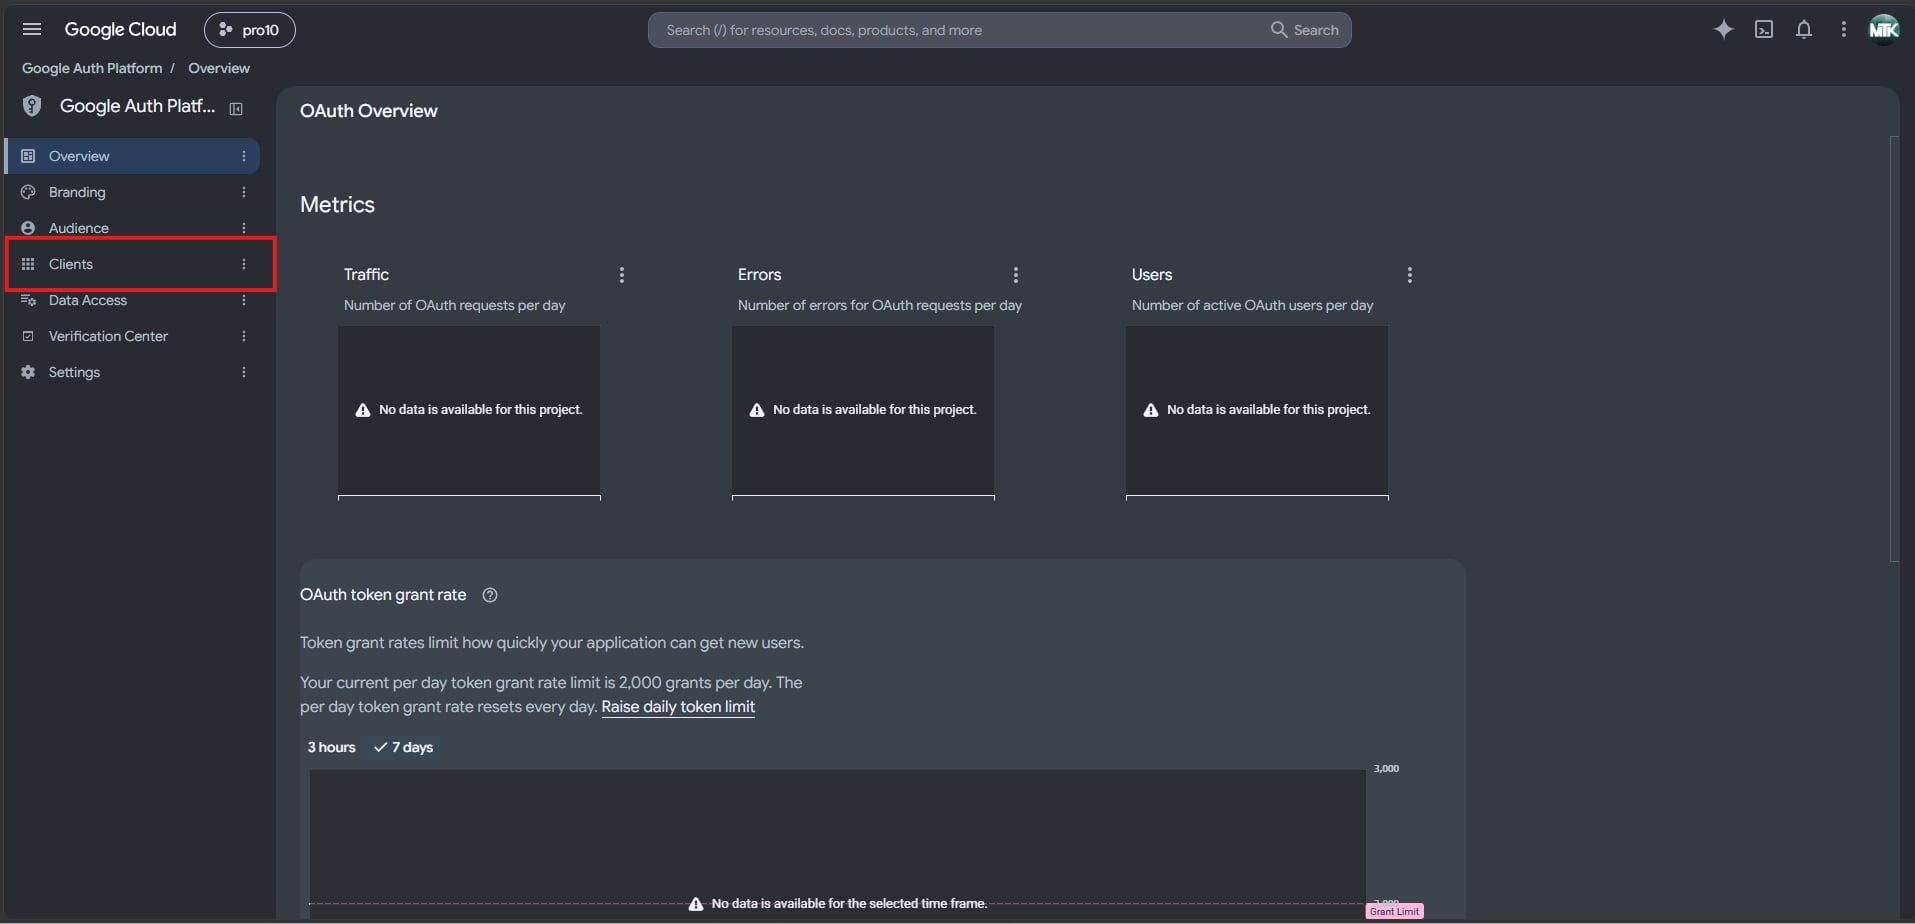
\includegraphics[width=\textwidth,height=0.30\textheight,keepaspectratio]{images/auth/auth-06.jpg}
    \caption{การเปิดเมนู Clients}
    \label{fig:auth-google-clients}
\end{figure}
\end{samepage}

\subsection{การสร้าง OAuth Client สำหรับ Web application}
\begin{samepage}
\noindent\textbf{ขั้นตอนที่ 7} ที่หน้า Clients กดปุ่ม Create client เพื่อเริ่มสร้าง OAuth Client
\begin{figure}[H]
    \centering
    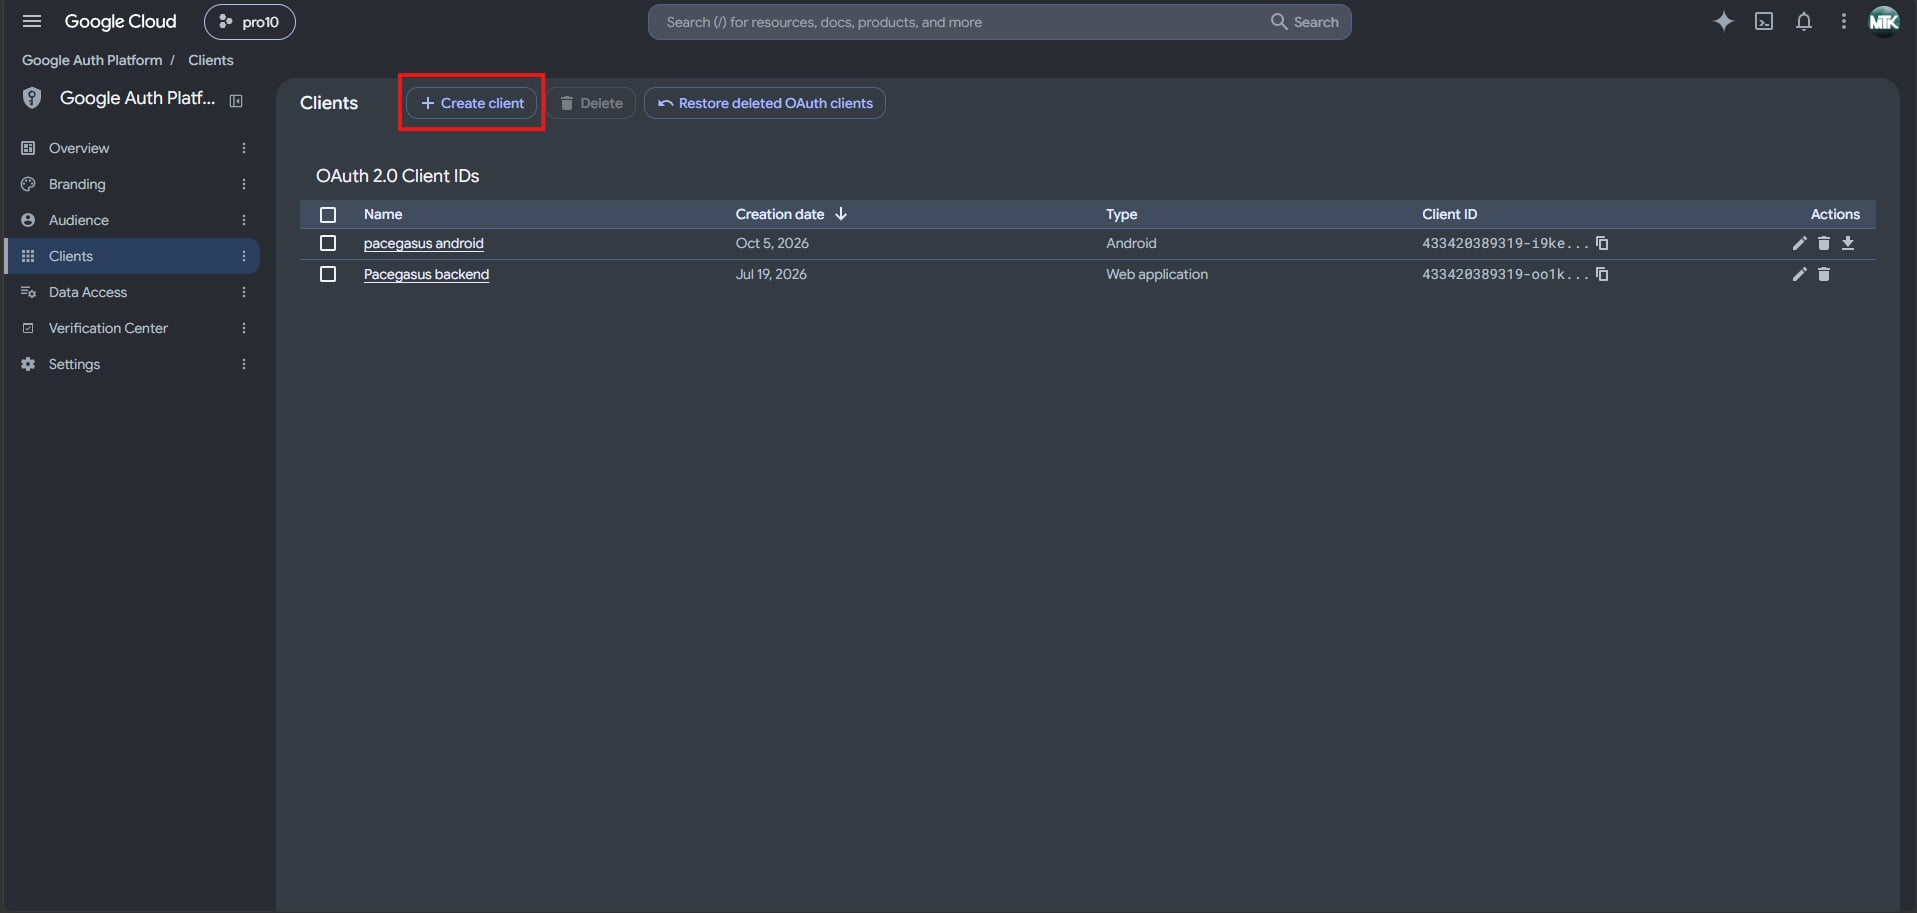
\includegraphics[width=\textwidth,height=0.30\textheight,keepaspectratio]{images/auth/auth-01.jpg}
    \caption{การเริ่มสร้าง OAuth Client}
    \label{fig:auth-google-create-client}
\end{figure}
\end{samepage}

\begin{samepage}
\noindent\textbf{ขั้นตอนที่ 8} เลือก Application type เป็น Web application และกำหนดชื่อ Client จากนั้นตั้งค่าที่อยู่ที่เกี่ยวข้องกับสภาพแวดล้อมของระบบก่อนกด Create
\begin{figure}[H]
    \centering
    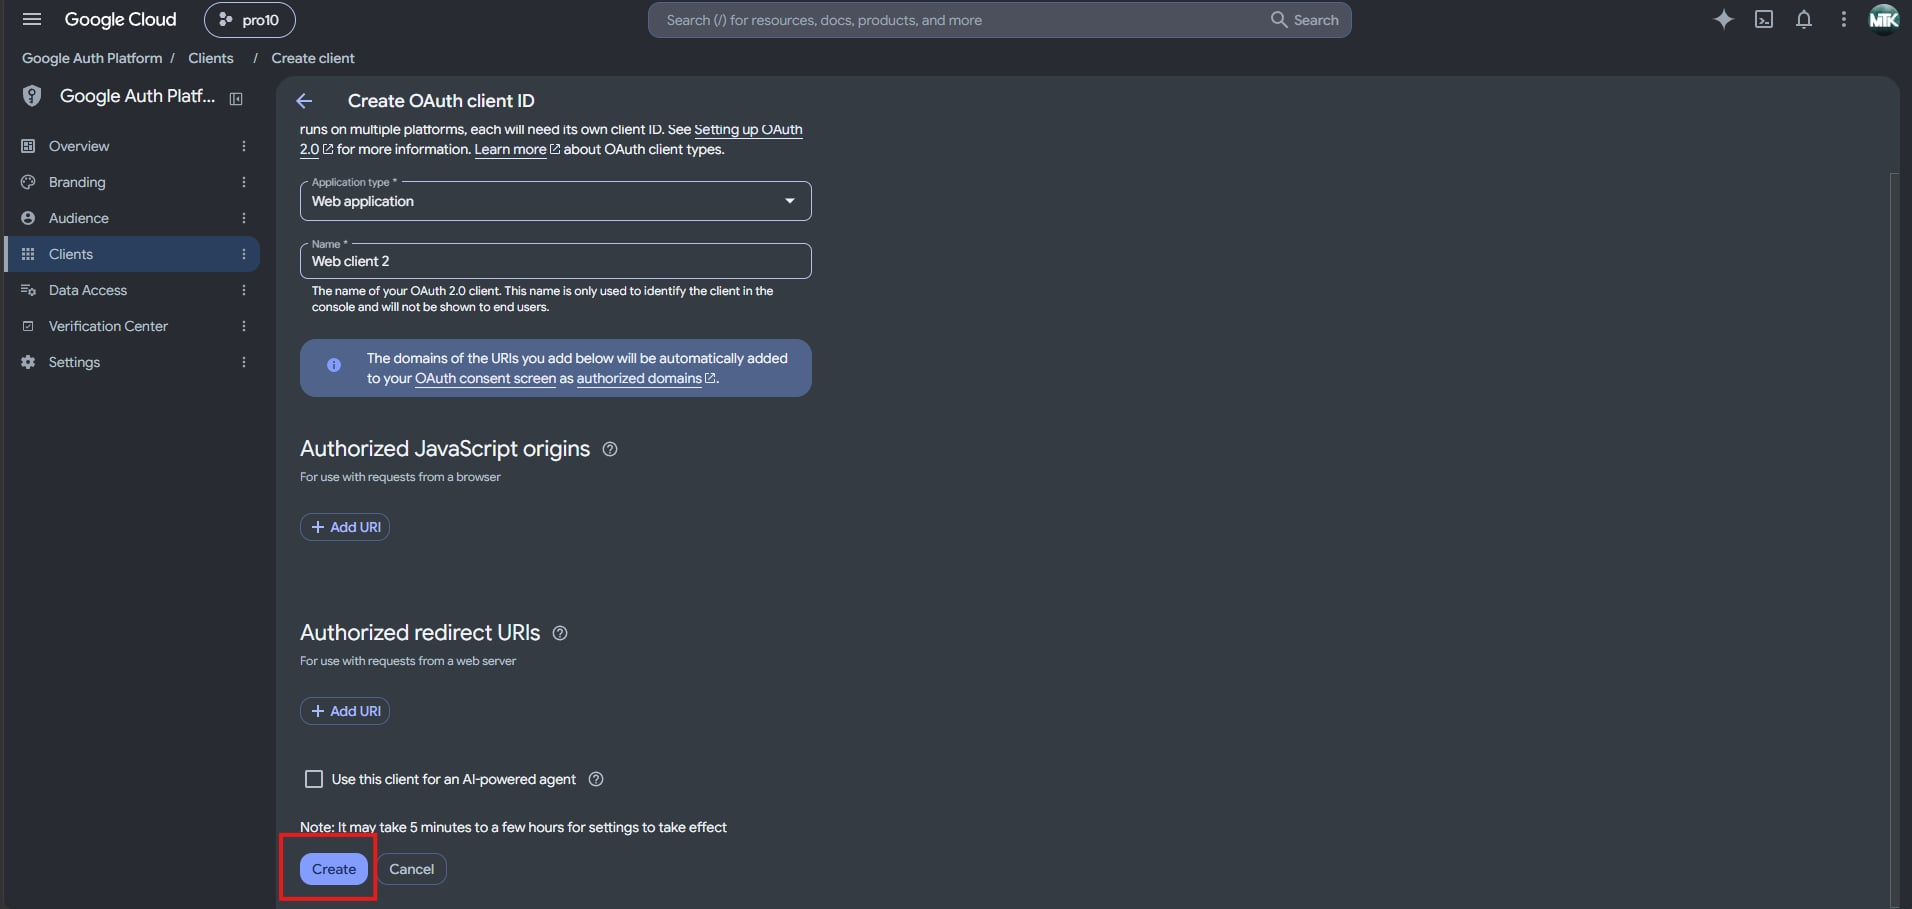
\includegraphics[width=\textwidth,height=0.30\textheight,keepaspectratio]{images/auth/auth-02.jpg}
    \caption{หน้าสร้าง OAuth Client แบบ Web application}
    \label{fig:auth-google-web-client}
\end{figure}
\end{samepage}

\begin{samepage}
\noindent\textbf{ขั้นตอนที่ 9} เมื่อมี Client ของระบบแล้ว ให้เลือกชื่อรายการประเภท Web application เพื่อเปิดรายละเอียด
\begin{figure}[H]
    \centering
    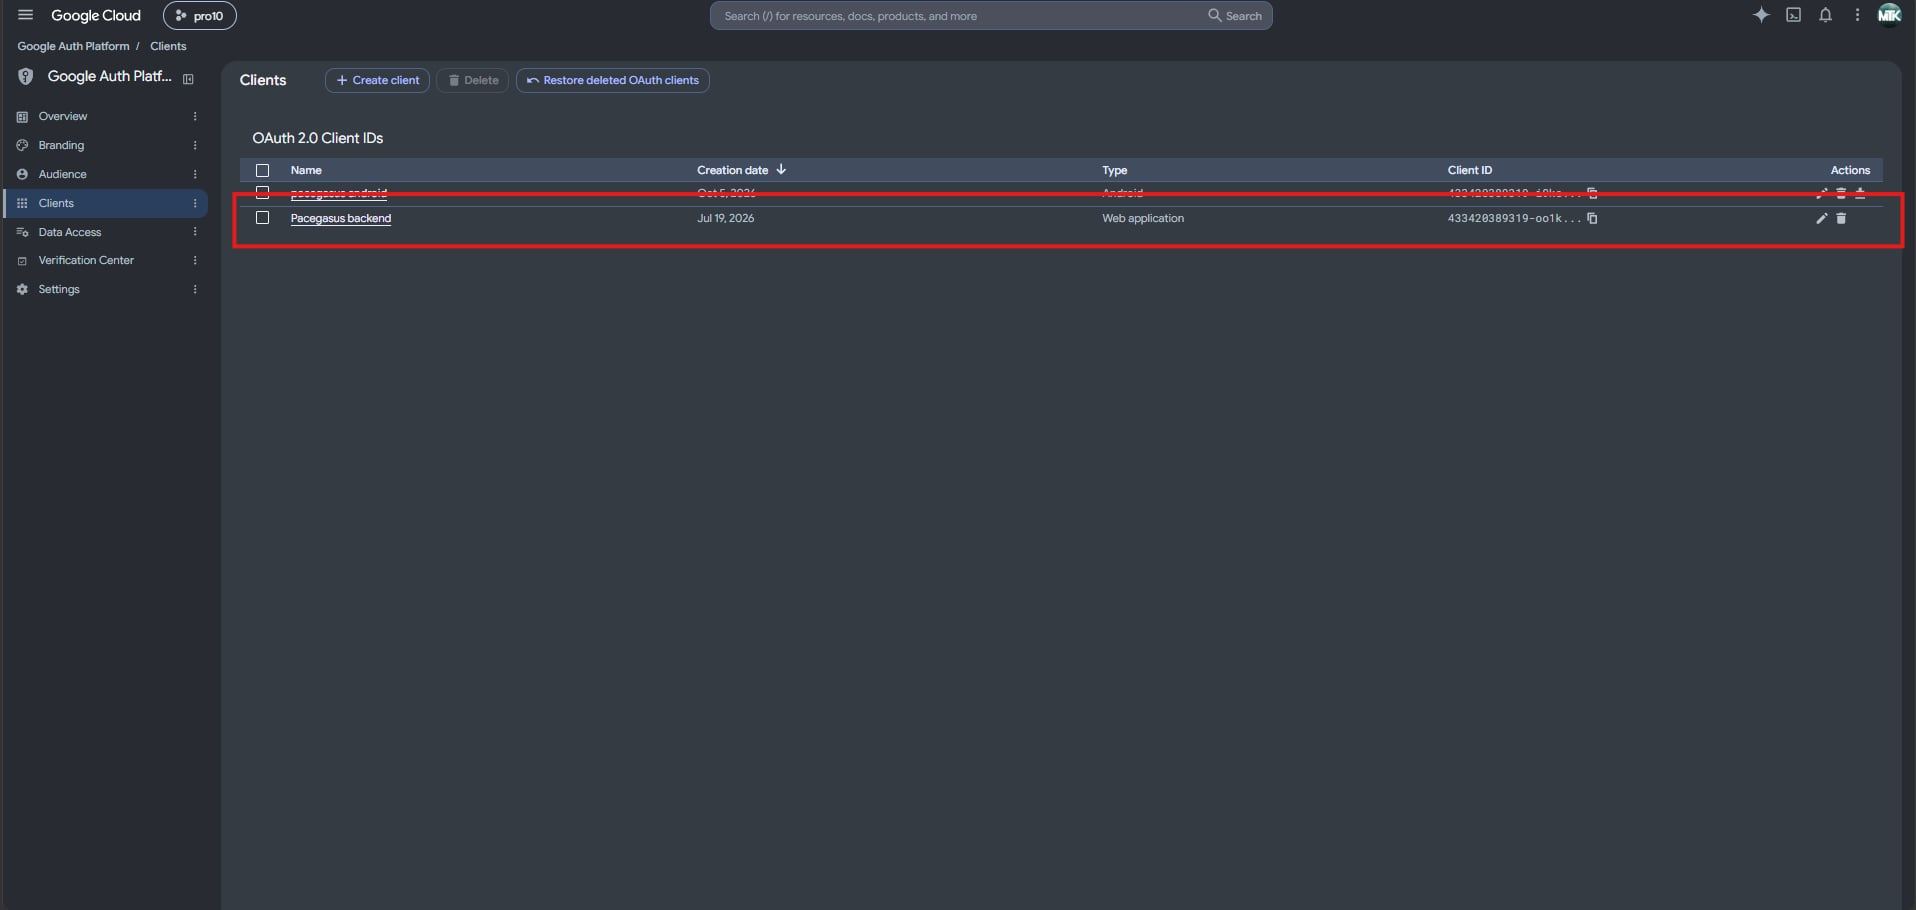
\includegraphics[width=\textwidth,height=0.30\textheight,keepaspectratio]{images/auth/auth-15.jpg}
    \caption{การเลือกรายการ Web application Client}
    \label{fig:auth-google-open-web-client}
\end{figure}
\end{samepage}

\begin{samepage}
\noindent\textbf{ขั้นตอนที่ 10} ดูตำแหน่ง Client ID ในส่วน Additional information สำหรับนำค่าของโครงการไปใช้ในการตั้งค่าการยืนยันตัวตน โดยค่าในภาพถูกปิดบังไว้
\begin{figure}[H]
    \centering
    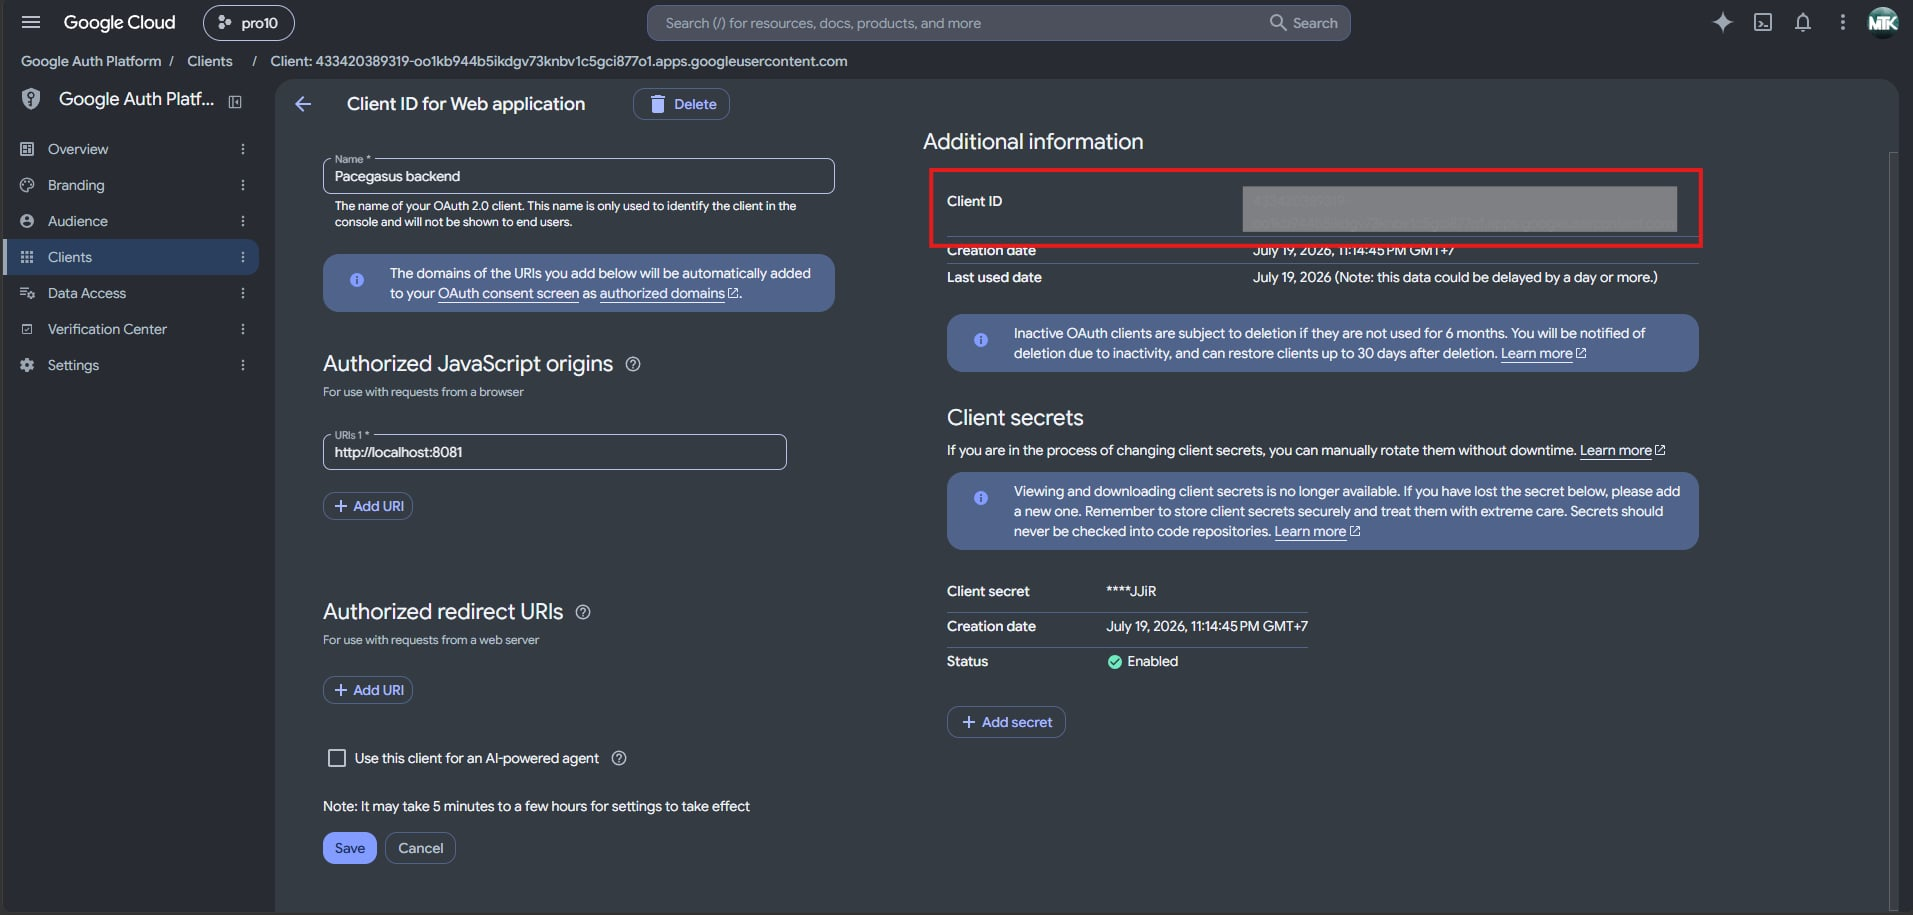
\includegraphics[width=\textwidth,height=0.30\textheight,keepaspectratio]{images/auth/auth-05.jpg}
    \caption{ตำแหน่ง Client ID ของ Web application}
    \label{fig:auth-google-client-id}
\end{figure}
\end{samepage}

\subsection{การสร้าง OAuth Client สำหรับ Android}
\begin{samepage}
\noindent\textbf{ขั้นตอนที่ 11} สร้าง Client อีกครั้งโดยเลือก Application type เป็น Android กำหนดชื่อ Client และกรอก Package name กับ SHA-1 certificate fingerprint ให้ตรงกับแอปพลิเคชันและใบรับรองที่ใช้ลงนาม จากนั้นกด Create
\begin{figure}[H]
    \centering
    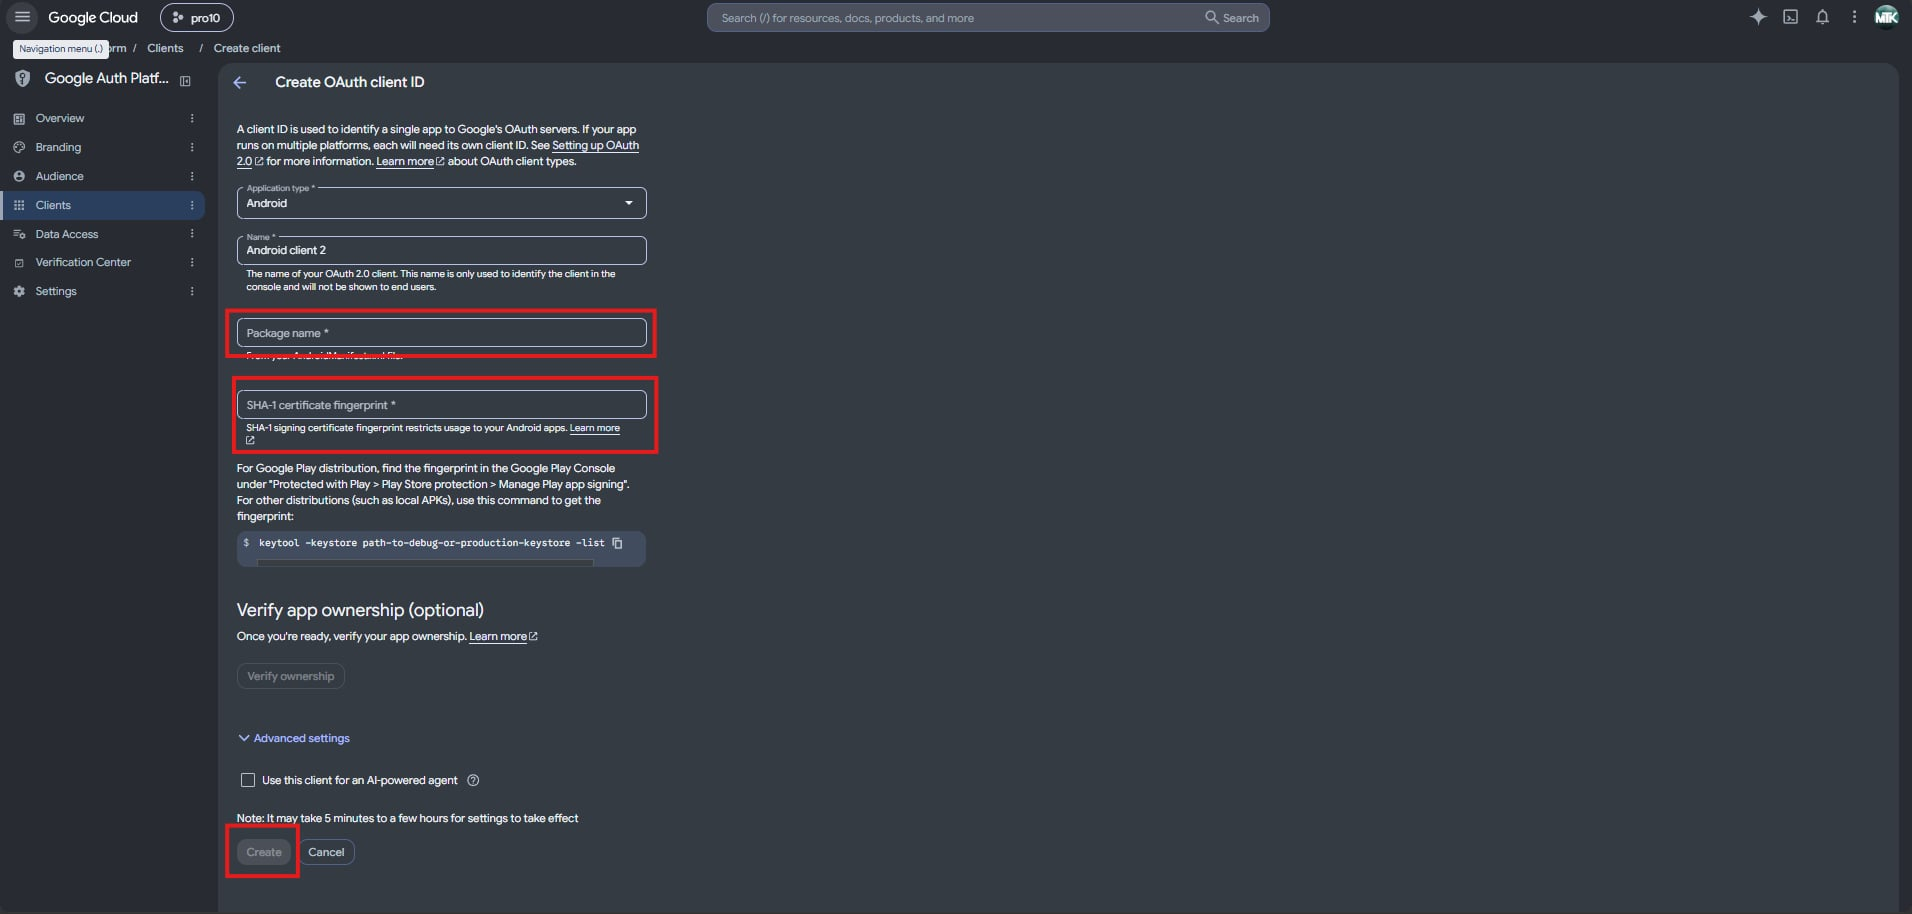
\includegraphics[width=\textwidth,height=0.30\textheight,keepaspectratio]{images/auth/auth-16.jpg}
    \caption{การสร้าง OAuth Client แบบ Android}
    \label{fig:auth-google-android-client}
\end{figure}
\end{samepage}

\subsection{การนำค่าการยืนยันตัวตนไปกำหนดในระบบ}
นำค่า Client ID ไปกำหนดในส่วนตั้งค่าการเข้าสู่ระบบของ Pacegasus ตามประเภท Client ที่ระบบใช้
ภาพชุดนี้แสดงตำแหน่งรับค่าจาก Google Cloud Console
ส่วนตำแหน่งไฟล์และตัวแปรสำหรับใส่ค่าในระบบจะเพิ่มจากโค้ดและภาพประกอบจริง
% TODO: เพิ่มภาพตั้งค่าหน้าความยินยอมและที่อยู่ redirect ของระบบจริง
% TODO: เพิ่มภาพการกำหนด Client ID และค่าที่เกี่ยวข้องในโครงการจริง
% TODO: เพิ่มภาพการเชื่อมต่อผู้ให้บริการ Google กับระบบยืนยันตัวตน หากระบบใช้ขั้นตอนดังกล่าว
% TODO: เพิ่มภาพทดสอบเข้าสู่ระบบสำเร็จหลังตั้งค่าครบ

\section{การตั้งค่า API แผนที่ Sphere GISTDA}
ส่วนนี้อธิบายการสร้างรายการ API Key และตรวจสอบ Project name
สำหรับนำไปตั้งค่าบริการแผนที่ของระบบ Pacegasus
ภาพประกอบเริ่มต้นหลังจากเข้าสู่บัญชี Sphere GISTDA แล้ว

\subsection{การเข้าสู่หน้าจัดการ API Keys}
\begin{samepage}
\noindent\textbf{ขั้นตอนที่ 1} เมื่อเข้าสู่หน้า Dashboard ของ Sphere GISTDA ให้เลือกเมนู API Keys ทางด้านซ้ายตามกรอบสีแดง
\begin{figure}[H]
    \centering
    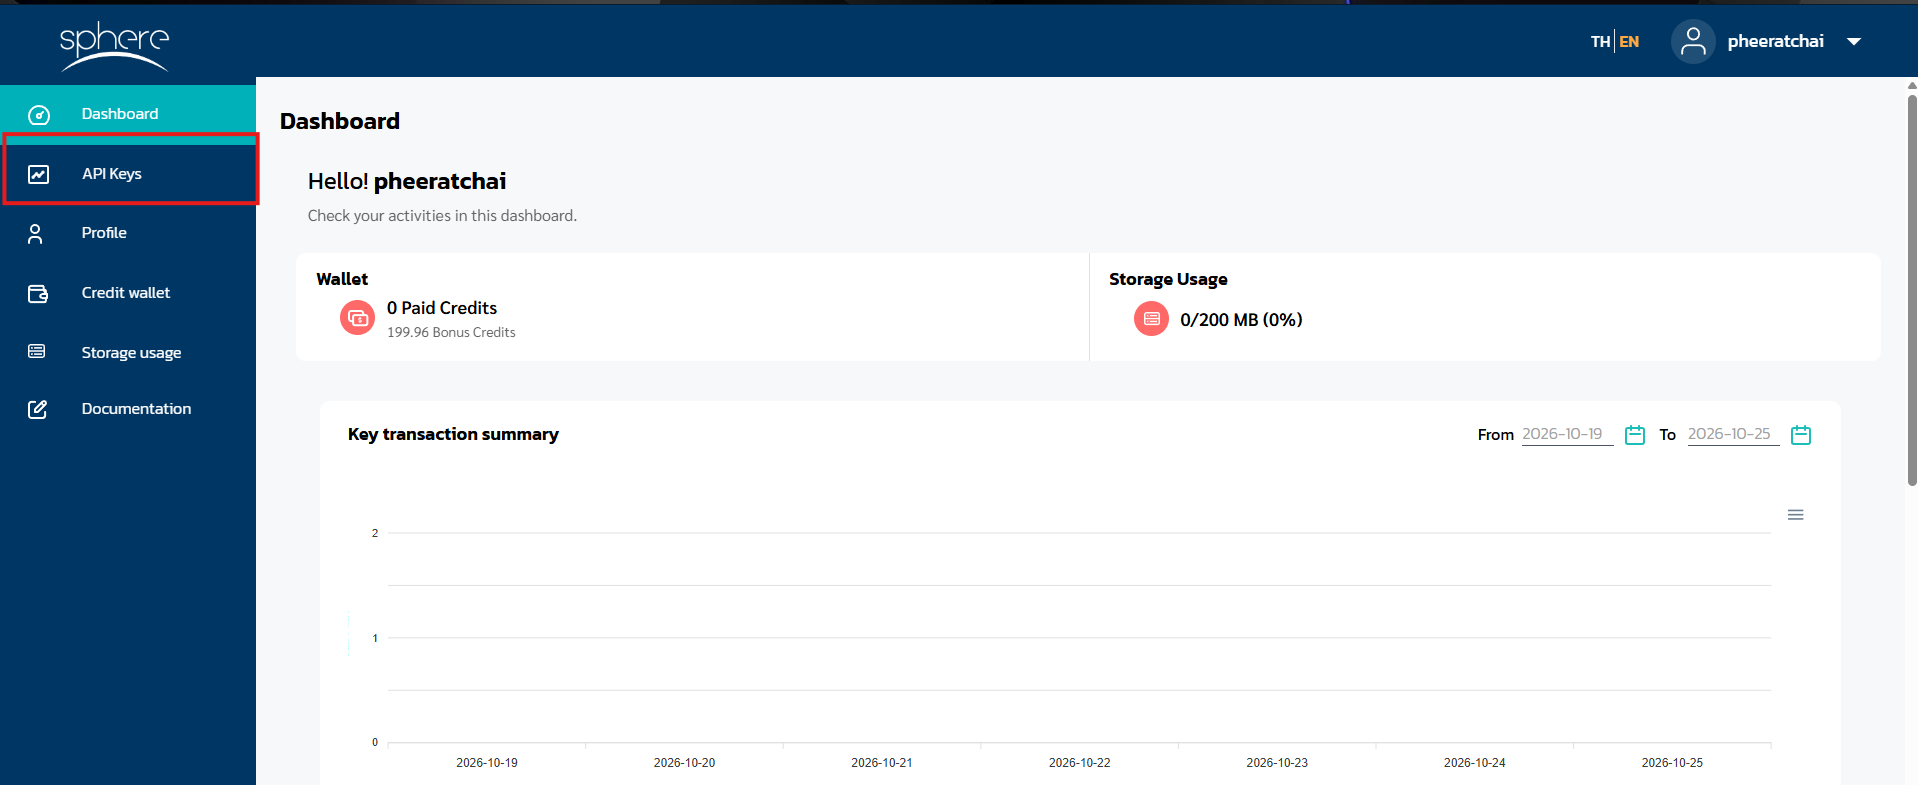
\includegraphics[width=\textwidth,height=0.30\textheight,keepaspectratio]{images/sphere/sphere-01.png}
    \caption{การเปิดเมนู API Keys ของ Sphere GISTDA}
    \label{fig:sphere-open-api-keys}
\end{figure}
\end{samepage}

\begin{samepage}
\noindent\textbf{ขั้นตอนที่ 2} ในหน้า API Keys Management ให้กดปุ่ม Create บริเวณด้านขวาบน เพื่อเปิดหน้าสร้าง API Key
\begin{figure}[H]
    \centering
    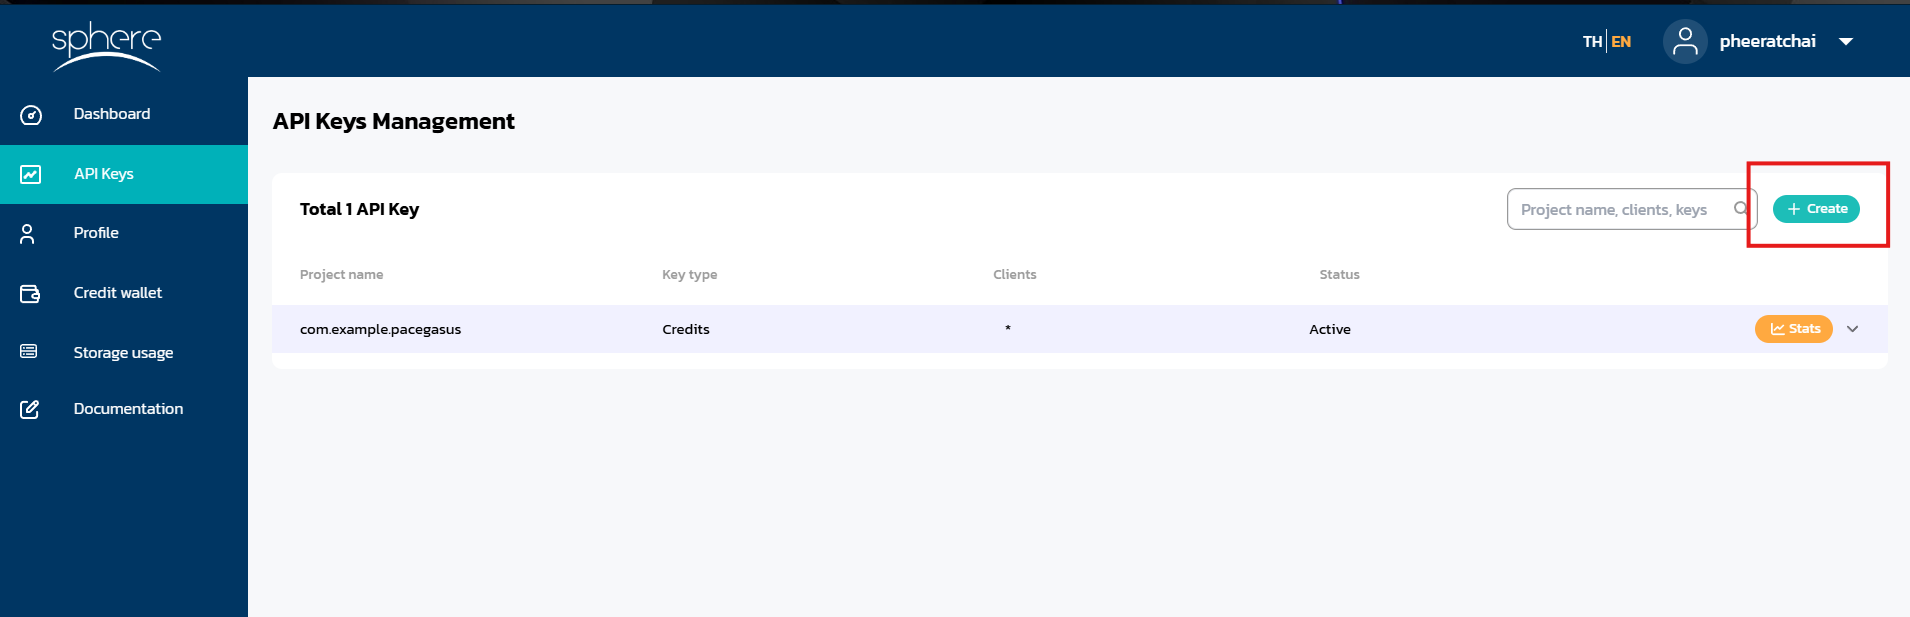
\includegraphics[width=\textwidth,height=0.30\textheight,keepaspectratio]{images/sphere/sphere-02.png}
    \caption{การเริ่มสร้าง API Key ของ Sphere GISTDA}
    \label{fig:sphere-create-api-key}
\end{figure}
\end{samepage}

\subsection{การกำหนด Project name และสร้าง API Key}
\begin{samepage}
\noindent\textbf{ขั้นตอนที่ 3} ในหน้าต่าง Create new API key ให้กรอก Project name ของโครงการ เช่น \texttt{com.example.pacegasus} จากนั้นกำหนด Clients และ Allowed IP ให้ตรงกับสภาพแวดล้อมที่ใช้งาน อ่านเงื่อนไข GISTDA sphere API Terms of Use และทำเครื่องหมายยอมรับก่อนกด Save
\begin{figure}[H]
    \centering
    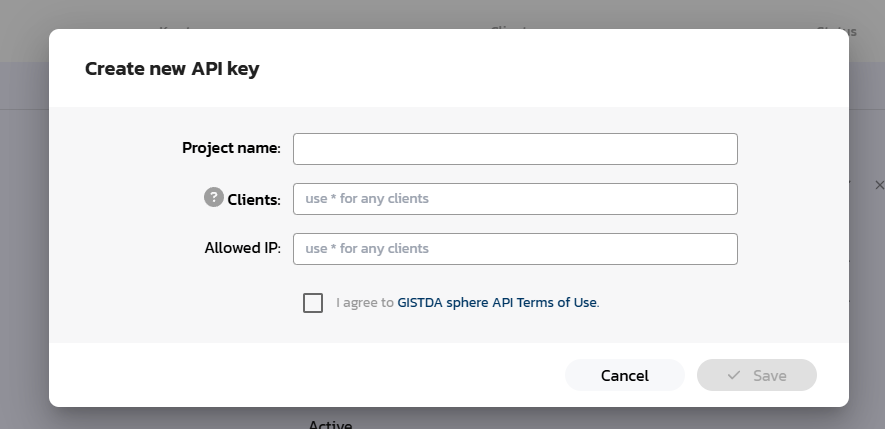
\includegraphics[width=\textwidth,height=0.30\textheight,keepaspectratio]{images/sphere/sphere-03.png}
    \caption{แบบฟอร์มกำหนด Project name และข้อมูล API Key}
    \label{fig:sphere-project-form}
\end{figure}
\end{samepage}

\subsection{การดูและคัดลอก API Key}
\begin{samepage}
\noindent\textbf{ขั้นตอนที่ 4} เมื่อบันทึกแล้ว ให้เปิดรายละเอียดรายการที่สร้างไว้ในหน้า API Keys Management ตรวจสอบช่อง Project name และกดไอคอนคัดลอกข้าง API Key เพื่อนำค่าไปตั้งค่าในระบบ โดยภาพตัวอย่างปิดบังคีย์บางส่วนไว้
\begin{figure}[H]
    \centering
    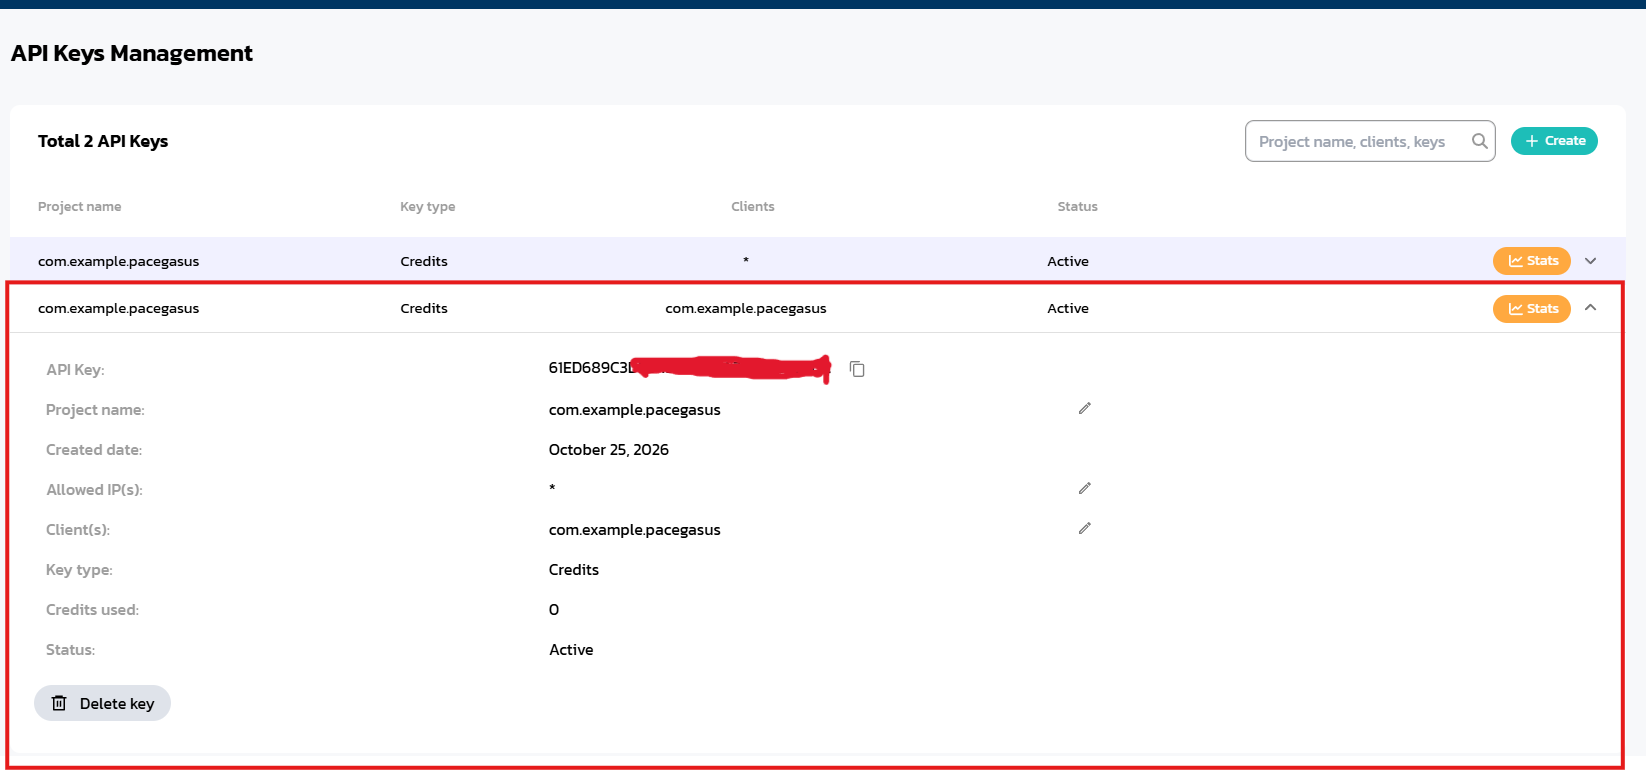
\includegraphics[width=\textwidth,height=0.30\textheight,keepaspectratio]{images/sphere/sphere-04.png}
    \caption{ตำแหน่ง Project name และ API Key ของ Sphere GISTDA}
    \label{fig:sphere-key-details}
\end{figure}
\end{samepage}

\subsection{การนำ Project name และ API Key ไปกำหนดในแอปพลิเคชัน}
บันทึก Project name และ API Key จากรายการเดียวกันไว้สำหรับตั้งค่าการเชื่อมต่อแผนที่ของ Pacegasus
โดยใช้ค่าของโครงการที่ผู้ติดตั้งสร้างขึ้นจริง
% TODO: เพิ่มภาพตำแหน่งไฟล์และชื่อตัวแปรที่ใช้กำหนด Project name และ API Key ในโค้ดจริง

\subsection{การทดสอบการแสดงผลแผนที่}
% TODO: เพิ่มขั้นตอนเปิดหน้าแผนที่และภาพผลหลังตั้งค่าในแอปพลิเคชันจริง

\section{การตั้งค่าการเชื่อมต่อบริการของระบบ}
% TODO: ระบุตำแหน่งกำหนด API URL และค่าที่เกี่ยวข้องตามไฟล์โครงการจริง

\section{การเรียกใช้งานและตรวจสอบหลังติดตั้ง}
% TODO: เพิ่มคำสั่งเรียกใช้งาน ภาพหน้าจอเริ่มต้น และผลที่แสดงว่าติดตั้งสำเร็จ
